
\begin{abstract}
Within the framework of this study the suitability of the \emph{Rust}
ecosystem for forensic tool development was evaluated. As case study,
the tool \emph{Strings­ext} was developed. Starting from analysing the
specific requirements of forensic software in general and those of the
present case study, all stages of the software development life-cycle
have been executed, up to the first production release.
\emph{Strings­ext} is a reimplementation and enhancement of the
\emph{GNU-strings} tool, a widely used program in forensic
investigations. \emph{Strings­ext} recognizes Cyrillic, CJKV characters
and other scripts in all supported multi-byte-encodings while
\emph{GNU-strings} fails in finding these in UTF-16 and other encodings.

During the case study it has become apparent that the \emph{Rust}
ecosystem provides good support for secure coding principles and unit
testing. Furthermore, the benchmarks showed a satisfactory performance
of the resulting \emph{Strings­ext} binaries comparable to the original
\emph{C} version.
\end{abstract}


\textbf{Special requirements in the field of digital
forensics}

\emph{Digital Forensics} also known as digital forensic science is a
branch of forensic science studying crime and its traces. ``Traces are
the most elementary information that results from crime. They are silent
witnesses that need to be detected, analysed, and understood to make
reasonable inferences about criminal phenomena, investigation or
demonstration for investigation and court purposes''
{[}\protect\hyperlink{meuwly2016}{2 p.~14}{]}. The branch science
dealing with digital traces and digitised information is referred as
\emph{digital forensic science}. It can be described as ``the process of
identifying, preserving, analysing and presenting digital evidence in a
manner that it legally acceptable.'' {[}\protect\hyperlink{guo2009}{3
p.~12}{]}. When digital traces are presented in court to support an
assertion the term \emph{digital evidence DE} or \emph{electronic
evidence} is in common use. In this work I use the term \emph{digital
evidence} following common practise in Great Britain.

Most human interaction with electronic devices leaves traces in some
electronic memory. In cases the user does not directly communicate with
its device additional traces may also be found in all intermediate
(network) devices. Due to the cross-linked nature of computer systems
the total amount of data that needs to be taken into consideration when
investigating a crime is enormous. In this ocean of information the
investigator has to find specific drops of information constituting
digital evidences. Furthermore, imagine someone throws a stone in the
sea. It will change the state of the water particles in various places,
but only a tiny share of this change is suitable to prove that the stone
was indeed thrown in water.

Following the principles in Transactional Analysis as founded by the
psychologist Eric Berne, the term ``transaction'' can be defined as the
smal­lest atomic interaction in a human - computer system communication.
For digital forensic practitioners the well-known and well documented
cause-effect relationships between human transactions and digital traces
is of utmost importance. A cause-effect-relationship is usually part of
a non linear chain of events. For example an attacker may send
"phishing" emails to its victims that try to lure them to
identity-stealing sites. The stolen identity is then sold and will be
used in other crimes. Behind the scenes many systems are involved in
such a scenario. A typical transaction of interest could be ``the user
has opened a browser window and visited the site xy'' which leaves
traces in some computer memory. In the domain of digital forensics an
observation of a well known cause-effect-relationship between an
electronic trace (effect) and what has happened (cause) is an called
\textbf{artefact}. It embodies any ``item of interest that help an
investigation move forward.'' {[}\protect\hyperlink{harichandran2016}{4
p.~125}{]}. A more formal definition named \emph{Curated (digital)
Forensic Artefact (CuFA)} proposed in
{[}\protect\hyperlink{harichandran2016}{4 p.~131}{]} embraces that it
must:

\begin{itemize}
\item
  be curated via a procedure which uses forensic techniques.
\item
  have a location in a useful format (when applicable).
\item
  have evidentiary value in a legal proceeding.
\item
  be created by an external force/artificially.
\item
  have antecedent temporal relation/importance.
\item
  be exceptional (based on accident, rarity, or personal interest).
\end{itemize}

Forensic examiners - the law enforcement personnel who deal with digital
evidence - face inter alia two challenges:

\begin{enumerate}
\def\labelenumi{\arabic{enumi}.}
\item
  to collect and to preserve the huge amount of data that may be related
  to a crime and
\item
  to search and identify artefacts in the collected data.
\end{enumerate}

The latter aspect includes so called \emph{string search} which is
useful when dealing with unknown binaries . Most executable binary code
contains human readable character sequences called strings. A very
common used program to extract strings from a binary executable code is
the so called \emph{GNU-strings} program. Also, the software tool
\emph{Stringsext} developed in this present work is made for this
purpose: The new development is designed to overcome some of
\emph{GNU-strings} shortcomings. Where possible, it maintains
\emph{GNU-strings'} user-interface.

\hypertarget{_tool_requirements_in_digital_forensics}{\section{Tool
Requirements in Digital
Forensics}\label{_tool_requirements_in_digital_forensics}}

This chapter describes general requirements towards forensic tools. They
partly emerge from legal and technical demands and motivate, inter alia,
the choice of the programming language Rust.

\hypertarget{_tool_validation}{\subsection{Tool
validation}\label{_tool_validation}}

Like in other established forensic disciplines the forensic soundness or
reliability of digital evidence is determined by the validity and
correctness of forensic software used in examination. In other words, to
guarantee that the digital evidence is forensically sound, all tools
used to collect, preserve and analyse digital evidences must be
validated. Tool validation can also be formally required to comply with
standards like the \emph{ISO 17025 Laboratory Accreditation standard}.

It should be noted that the forensic community's definition of
\emph{validation} and \emph{verification} differs from what used in
software engineering. Two commonly used definitions state the following:

A short and catchy definition was proposed by Beckett and Slay
{[}\protect\hyperlink{beckett2007}{5}{]}:

\begin{description}
\item[Validation]
is the confirmation by examination and the provision of objective
evidence that a tool, technique or procedure functions correctly and as
intended.
\item[Verification]
is the confirmation of a validation with a laboratories tools,
techniques and procedures.
\end{description}

It means that establishing a reliable technical method to observe a
cause and effect relation between a human action and a resulting
artefact is called \emph{validation}. The test, whether a technical
device is suitable or not to execute the above method reliably, is
called \emph{verification}.

Craiger {[}\protect\hyperlink{craiger2006}{6 p.~92}{]} defines
\emph{validation} and \emph{verification} as follows:

\begin{description}
\item[Software verification]
provides objective evidence that the design outputs of a particular
phase of the software development life cycle meet all the specified
requirements for that phase. \emph{Software verification} looks for
\textbf{consistency, completeness, and correctness of the software and
its supporting documentation, as it is being developed}, and provides
support for a subsequent conclusion that software is validated. Software
testing is one of many verification activities intended to confirm that
software development output meets its input requirements. Other
verification activities include various static and dynamic analyses,
code and document inspections, walkthroughs, and other techniques.
\item[Software validation]
is a part of the design \textbf{validation for a finished
device}\ldots{}​considers software validation to be `confirmation by
examination and provision of objective evidence that software
specifications conform to user needs and intended uses, and that the
particular requirements implemented through software can be consistently
fulfilled.' In practice, software validation activities may occur both
during, and as at the end of the software development life cycle to
ensure that all requirements have been fulfilled. \ldots{}​the
validation of software typically includes \textbf{evidence that all
software requirements have been implemented correctly and completely}
and are traceable to system requirements. A conclusion that software is
validated is highly dependent upon comprehensive software testing,
inspections, analyses, and other verification tasks performed at each
stage of the software development life cycle.
\end{description}

Common to both definitions of validation is the mapping of the tool's
requirements to tests confirming that they fully and correctly
implemented. At first glance the above approach might seem simple to
implement but in many cases it is impossible to carry out:

\begin{quote}
Traditional research discourse on tool testing in this discipline
concerns validation of a tool, that is, all the functions of a tool, and
with the failure of a validation of a tool the traditional thinking is
to invalidate the tool. In most cases forensic tools are quite complex
and provide hundreds of specific functions, of which only a few may ever
be used by an examiner. Even trivial testing of all functions of a
forensic tool for every version under all conditions, conservative
estimates would indicate significant cost
{[}\protect\hyperlink{beckett2007}{5}{]}.
\end{quote}

To cope with this difficulty Beckett and Slay
{[}\protect\hyperlink{beckett2007}{5}{]} suggest a model so called
\emph{Model of tool neutral testing} or \emph{functionality oriented
validation}. Instead of testing if a software product meets all its
requirements an independent set of forensic functions and their
specifications is defined. This allows to decouple the validation
procedure from the implementation of the forensic tool itself. A
forensic function is an activity required in forensic investigation that
produces known valid results for a given set of test cases.

\begin{figure}[htbp]
\centering
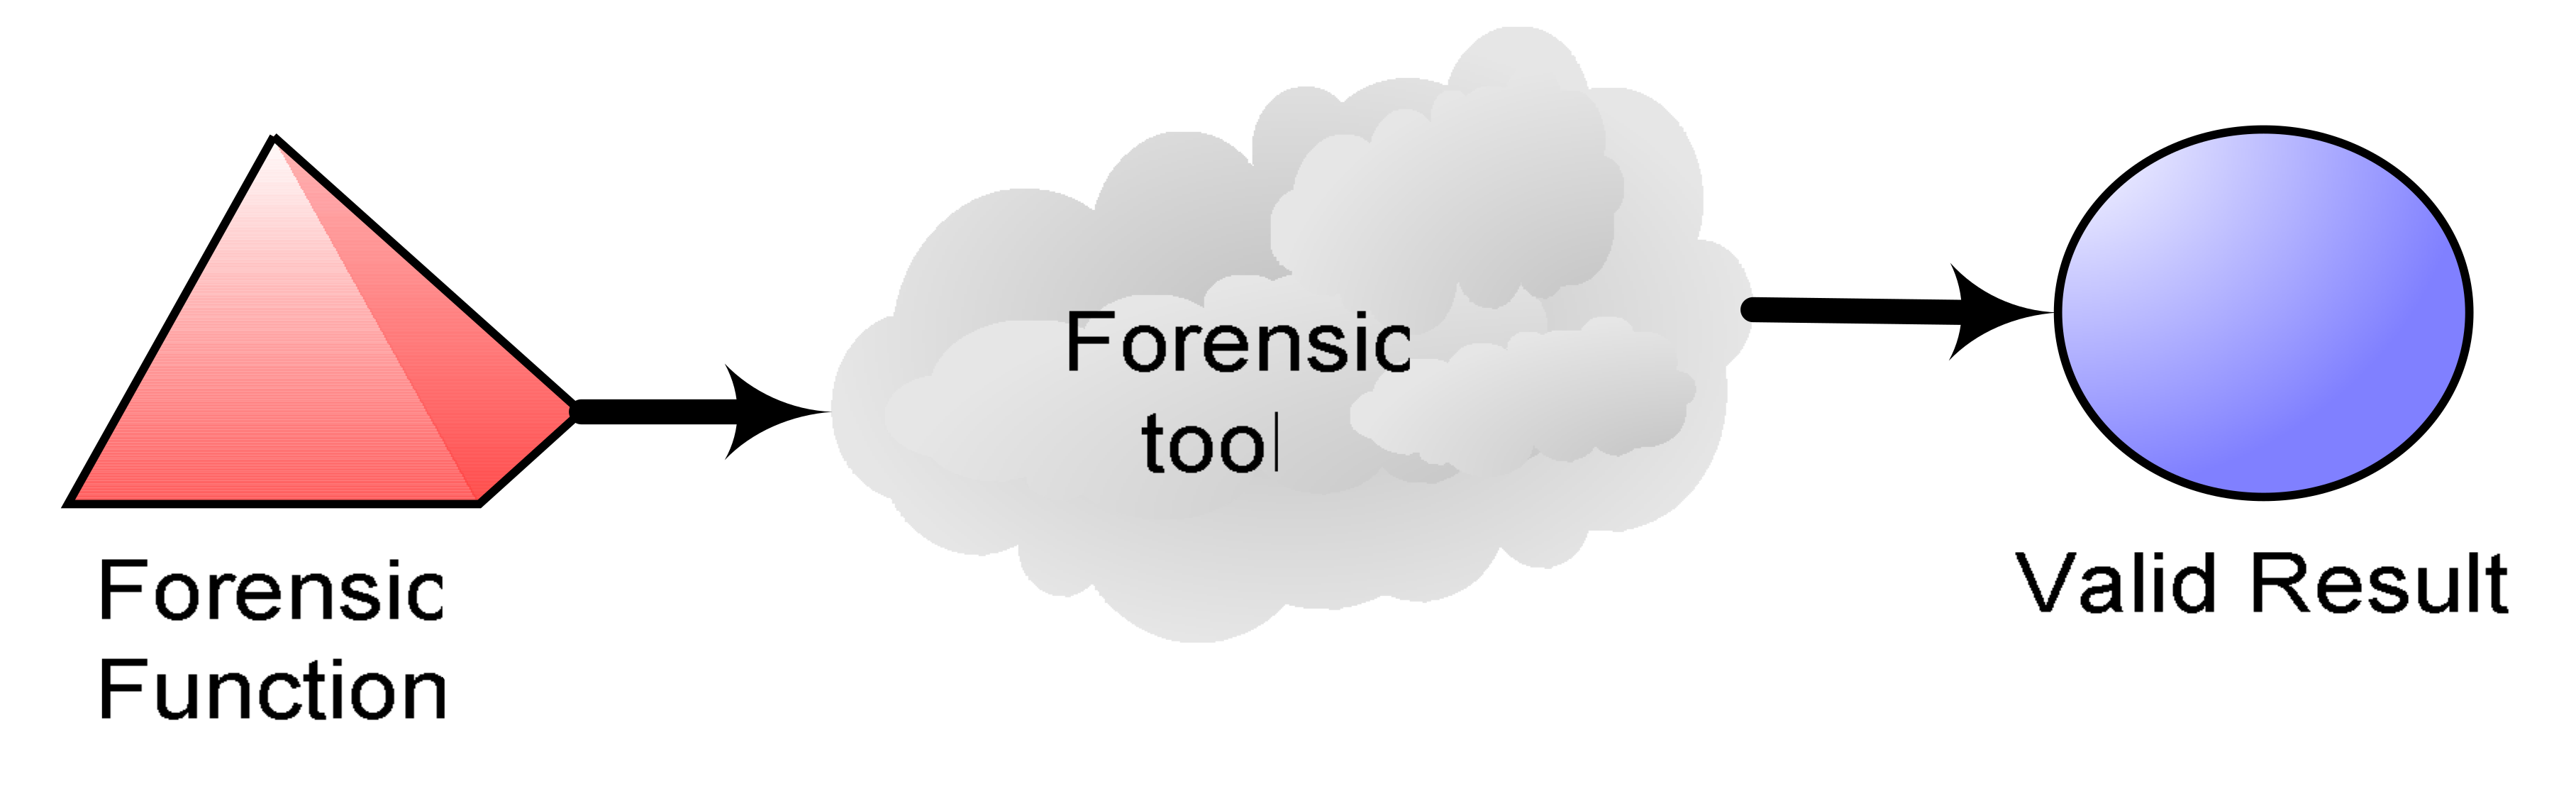
\includegraphics[width=0.80000\textwidth]{images/model_of_tool_neutral_testing.png}
\caption{Model of tool neutral testing}
\end{figure}

The first difficulty consists in breaking down the multitude of
activities in forensic investigation in function categories and
subcategories as shown in
\protect\hyperlink{an-overview-of-searching-function}{figure\_title}
{[}\protect\hyperlink{guo2009}{3 p.~17}{]}.

\begin{figure}[htbp]
\centering
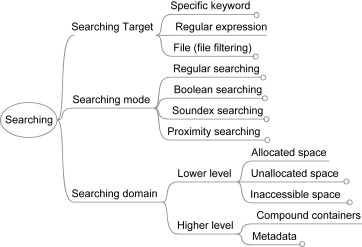
\includegraphics[width=0.60000\textwidth]{images/02-An_overview_of_searching_function.jpg}
\caption{An overview of searching function}
\end{figure}

The search target mapping as shown below illustrates under the
subcategory ``Character encoding'' the main deficit of
\emph{GNU-strings} supporting only ASCII encoding. In global cyberspace
forensic tools must identify a multitude of encodings. This leads us to
the main motivation and requirement of \emph{Strings­ext}:
\protect\hyperlink{character-encoding-support}{section\_title}

\begin{figure}[htbp]
\centering
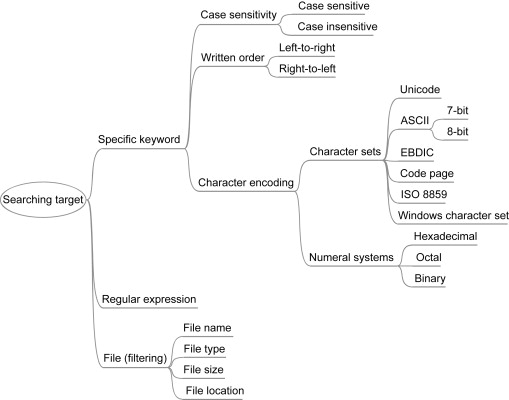
\includegraphics[width=0.80000\textwidth]{images/03-The_search_target_mapping.jpg}
\caption{The search target mapping}
\end{figure}

The \emph{functionality oriented validation} can be classified as
``black box testing'' examining functionality without any knowledge of
internal implementation, without seeing the source code. ``Black box
testing'' of functions and their specifications allows conducting
numerous tests with acceptable costs. It requires test cases with known
valid results. With \emph{Strings­ext} this approach is used to test the
correctness of the implementation when dealing with large real-world
data (cf.
\protect\hyperlink{functionality-oriented-validation}{section\_title}).

When the internal computation is as complex as in \emph{Strings­ext},
``white box testing'' is essential. The method chosen in the present
development ``test harness'' is detailed in the
\protect\hyperlink{automated-test-framework}{section\_title}.

\hypertarget{security1}{\subsection{Security}\label{security1}}

The relation between the criminal and the forensic examiner can be
described as follows: ``Make it hard for them to find you and impossible
for them to prove they found you''
{[}\protect\hyperlink{berinato2007}{7}{]}. Have your recognised the
statement? Is widely cited when it comes to define anti-forensics. This
traditional "hide and seek" relation might soon take a new dimension:
Eggendorfer {[}\protect\hyperlink{eggendorfer2016}{8}{]} stresses with
good reasons that forensic tools are software too and therefor
vulnerable to attacks.

\emph{GNU-strings} is part of the \emph{GNU binutils} collection which
became publicly available in 1999
{[}\protect\hyperlink{strings1999}{9}{]}. Today it has reached the
notable age of 17 years. \emph{GNU-strings} is a comparatively small
program with 724 lines of code only. It is all the more surprising that
in 2014 the security researcher Zalewski discovered a serious security
vulnerability \emph{CVE-2014-8485}
{[}\protect\hyperlink{zalewski2014}{10}{]}.

\begin{quote}
The setup\_group function in \texttt{bfd/elf.c} in \texttt{libbfd} in
GNU binutils 2.24 and earlier allows remote attackers to cause a denial
of service (crash) and possibly execute arbitrary code via crafted
section group headers in an ELF file.

---  CVE-2014-8485
\end{quote}

Zalewski headlined his bug report ``Don't run strings on untrusted
files.'' Needless to say that this advice can not be followed in the
context of a forensic investigation. In the meantime the bug was fixed
but users remain confused and bewildered.

The above bug is part of a vulnerability class related to memory safety
problems. \emph{GNU strings} is written in C, a language whose
abstractions can not guarantee memory savety. In order to exclude
potential vulnerabilities of the same kind from the start,
\emph{Strings­ext} was developed with the \emph{Rust} programming
language which is discussed further in the
\protect\hyperlink{rust}{???}.

\hypertarget{_code_efficiency}{\subsection{Code
efficiency}\label{_code_efficiency}}

The searching domain in forensic investigations is often as large as the
seized data-carrier. Nowadays hard-disk images hold several TiB of data.
Memory images of the RAM are smaller, but still some GiB in size. In
order to address so big search domains, forensic software must operate
very efficiently. This is why forensic software is often programmed in C
or C++. But not only the programming language matters: Efficient code
requires carefully chosen abstractions, efficient algorithms avoiding
un­ne­ces­sary data-copies and program-loops.

\hypertarget{strings-and-forensics}{\section{\texorpdfstring{\emph{GNU-strings}
in forensic
examination}{GNU-strings in forensic examination}}\label{strings-and-forensics}}

This chapter first analyses \emph{GNU-strings'} limitations concerning
multi-byte-encodings and international scripts (cf.
\protect\hyperlink{test-case-strings}{section\_title}). Further, a use
case shows how \emph{GNU-strings} is typically used in forensic
examination (cf: \protect\hyperlink{_typical_usage}{section\_title}).
Based upon this we derive a set of requirements for \emph{Strings­ext}
(cf:
\protect\hyperlink{_requirements_derived_from_typical_usage}{section\_title}).

Forensic examiners use the GNU program \emph{strings} to get a sense of
the functionality of an unknown program. E.g. extracted URLs to
malicious sites can be an indicator of malware. Also, user prompts,
error messages, and status messages can give hints for further
investigation.

\hypertarget{test-case-strings}{\subsection{Test case 1 - International
character encodings}\label{test-case-strings}}

As discussed above the main motivation for developing \emph{Strings­ext}
are the missing multi-byte character encoding semantics in
\emph{GNU-strings}. \emph{GNU-strings} encoding support consists of a
rudimentary filter accessed with the option \texttt{-\/-encoding}. For
details see the \protect\hyperlink{legend-strings}{table\_title}. How
well does \emph{GNU-strings} detect Unicode?

The
\protect\hyperlink{test-international-character-encodings}{figure\_title}
shows the content of a text file chosen as test case.

\begin{figure}[htbp]
\centering
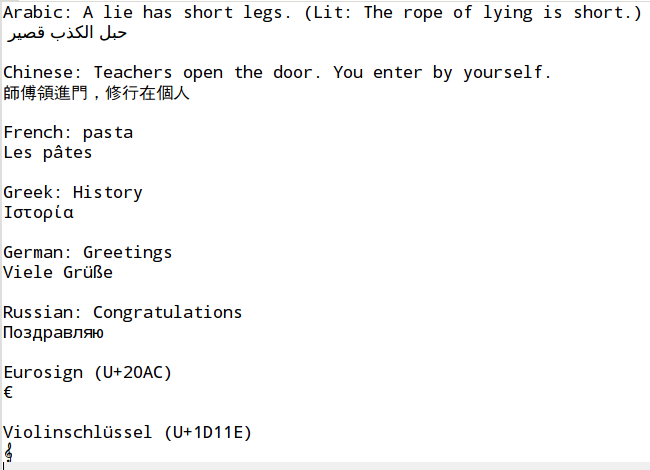
\includegraphics[width=0.80000\textwidth]{images/test_case_encoding-input.png}
\caption{Test case international character encodings}
\end{figure}

The above file is then is converted into different encodings using the
following script:

\textbf{Test case preparation.}

\begin{Shaded}
\begin{Highlighting}[]
\CommentTok{#!/bin/sh}
\FunctionTok{cp} \NormalTok{orig.txt encoded-utf8.txt}
\ExtensionTok{iconv} \NormalTok{-f utf8 -t utf16le orig.txt }\OperatorTok{>}\NormalTok{encoded-utf16le.txt}
\ExtensionTok{iconv} \NormalTok{-f utf8 -t utf32le orig.txt }\OperatorTok{>}\NormalTok{encoded-utf32le.txt}
\ExtensionTok{iconv} \NormalTok{-f utf8 -t utf16be orig.txt }\OperatorTok{>}\NormalTok{encoded-utf16be.txt}
\ExtensionTok{iconv} \NormalTok{-f utf8 -t utf32be orig.txt }\OperatorTok{>}\NormalTok{encoded-utf32be.txt}
\end{Highlighting}
\end{Shaded}

In order to observe \emph{GNU-strings} Unicode detection capabilities,
all the above test-files are searched for valid graphic strings with the
command \texttt{strings} using all possible variation of its encoding
filter.

The following figures show \emph{GNU-strings} output.

\begin{figure}[htbp]
\centering
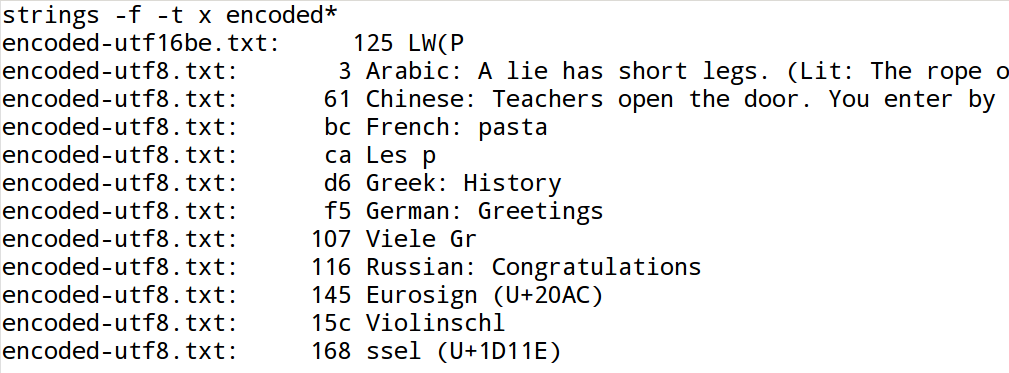
\includegraphics[width=0.80000\textwidth]{images/strings.png}
\caption{GNU-strings, single-7-bit}
\end{figure}

\begin{figure}[htbp]
\centering
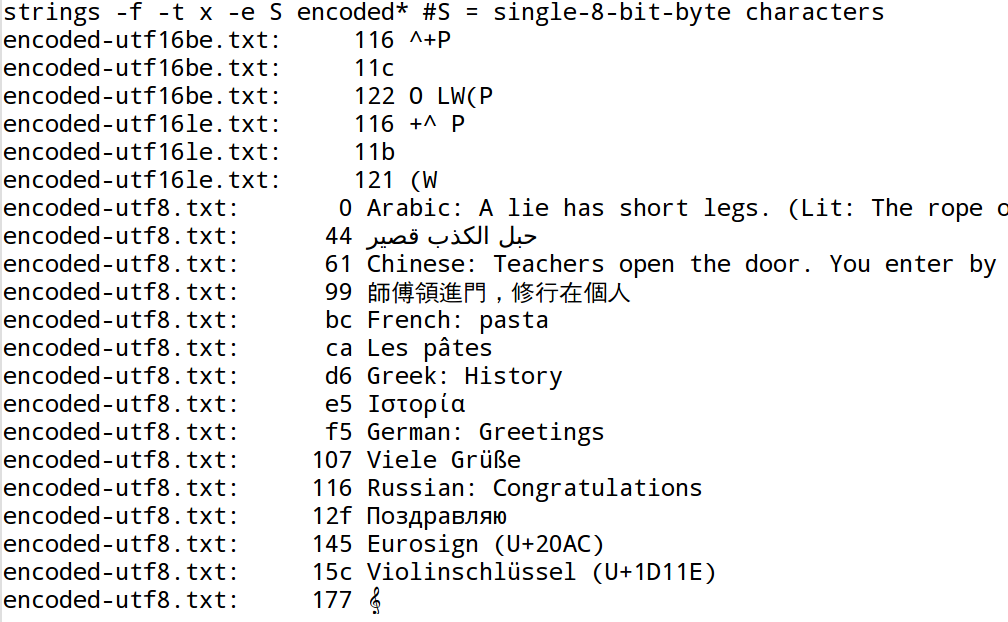
\includegraphics[width=0.80000\textwidth]{images/strings_-e_S.png}
\caption{GNU-strings, single-8-bit option}
\end{figure}

\begin{figure}[htbp]
\centering

\includegraphics[width=0.80000\textwidth]{images/strings_-e_l.png}
\caption{GNU-strings, 16-bit little-endian option}
\end{figure}

\begin{figure}[htbp]
\centering

\includegraphics[width=0.80000\textwidth]{images/strings_-e_b.png}
\caption{GNU-strings, 16-bit big-endian option}
\end{figure}

\begin{figure}[htbp]
\centering

\includegraphics[width=0.80000\textwidth]{images/strings_-e_L.png}
\caption{GNU-strings, 32-bit little-endian option}
\end{figure}

\begin{figure}[htbp]
\centering
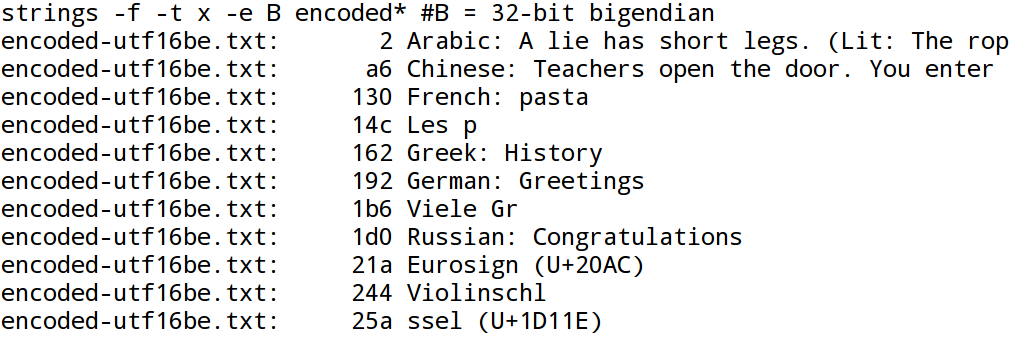
\includegraphics[width=0.80000\textwidth]{images/strings_-e_B.png}
\caption{GNU-strings, 32-bit big-endian option}
\end{figure}

\textbf{Results.}

As shown in the \protect\hyperlink{strings-e-capitals}{figure\_title},
the encoding filter \texttt{-e\ S} is the only filter that finds
international characters at all.

\begin{quote}
\textbf{Important}

\emph{UTF-8} is the only encoding in which \emph{GNU strings} is able to
find international characters.
\end{quote}

The \protect\hyperlink{strings-e-l}{figure\_title} and the
\protect\hyperlink{strings-e-b}{figure\_title} confirm that with
\emph{UTF-16} no international characters are recognized. The same holds
true for \emph{UTF-32}: see
\protect\hyperlink{strings-e-capitall}{figure\_title} and
\protect\hyperlink{strings-e-capitalb}{figure\_title}. This limitation
is of particular importance in forensic investigations: The
Microsoft-Windows operating system handles Unicode characters in memory
as 2 byte \emph{UTF-16} words. As a result when dealing with
Microsoft-Windows memory images, \emph{GNU-strings} is not able to
detect any international characters!

It should not be forgotten that \emph{GNU-strings} can not analyse
multi-byte encodings in general. This is why other very common encodings
e.g. \emph{big5} or \emph{koi8-r} were not tested even though they are
widely used.

The above-outlined limitations led to \emph{Strings­ext}'s main
requirement:
\protect\hyperlink{character-encoding-support}{section\_title}.

\hypertarget{_typical_usage}{\subsection{Typical
usage}\label{_typical_usage}}

The following script \footnote{The script was kindly provided by an
  employee of the German CERT.} shows how forensic examiners typically
use the program \emph{GNU-strings`}:

\textbf{Typical usage of GNU-strings.}

\begin{Shaded}
\begin{Highlighting}[]
\CommentTok{#!/bin/bash}
\FunctionTok{strings} \NormalTok{-a -t d }\VariableTok{$1} \OperatorTok{>} \VariableTok{$1}\NormalTok{.strings.temp           }
\FunctionTok{strings} \NormalTok{-a -t d -e l }\VariableTok{$1} \OperatorTok{>>} \VariableTok{$1}\NormalTok{.strings.temp   }
\FunctionTok{strings} \NormalTok{-a -t d -e L }\VariableTok{$1} \OperatorTok{>>} \VariableTok{$1}\NormalTok{.strings.temp}
\FunctionTok{strings} \NormalTok{-a -t d -e b }\VariableTok{$1} \OperatorTok{>>} \VariableTok{$1}\NormalTok{.strings.temp}
\FunctionTok{strings} \NormalTok{-a -t d -e B }\VariableTok{$1} \OperatorTok{>>} \VariableTok{$1}\NormalTok{.strings.temp}
\FunctionTok{strings} \NormalTok{-a -t d -e s }\VariableTok{$1} \OperatorTok{>>} \VariableTok{$1}\NormalTok{.strings.temp}
\FunctionTok{strings} \NormalTok{-a -t d -e S }\VariableTok{$1} \OperatorTok{>>} \VariableTok{$1}\NormalTok{.strings.temp}
\FunctionTok{sort} \NormalTok{-n -u -b }\VariableTok{$1}\NormalTok{.strings.temp }\OperatorTok{>} \VariableTok{$1}\NormalTok{.strings      }
\FunctionTok{rm} \VariableTok{$1}\NormalTok{.strings.temp                           }
\end{Highlighting}
\end{Shaded}

Please refer to \protect\hyperlink{legend-strings}{table\_title} for
details about the used options above.

The first and only parameter of the above script \texttt{\$1} is the
filename of the binary data to be examined.

\begin{itemize}
\item
  The examination is carried out by the \texttt{strings} command.
  \texttt{strings} is invoked in total seven times. Each run it scans
  the whole data, searches for valid graphic ASCII strings and appends
  its result to the temporary file \texttt{\$1.strings.temp}.
\item
  \texttt{-a} means that the whole file is to be scanned, not only a
  part of it.
\item
  The option \texttt{-t\ d} means that each line of output is prepended
  by the decimal offset indicating the location of the string that is
  found.
\item
  Even though \texttt{strings} can only recognise pure ASCII encodings
  the option \texttt{-e} allows specifying some variations concerning
  the memory layout in which the characters are stored. For example
  \texttt{-e\ b} means that one ASCII character is stored in two bytes
  (16 bit) in Big-Endian order. For the other variants please refer to
  \protect\hyperlink{legend-strings}{table\_title}.
\item
  It may surprise that \texttt{strings} with \texttt{-t\ d} is set up to
  print the offset in decimal although hexadecimal notation is generally
  preferred when dealing with binary data. The reason lies in the
  post-treatment performed in this line: The \texttt{-n} or
  \texttt{-\/-numeric-sort} option tells the \texttt{sort} command to
  interpret the beginning of the line as decimal number and sort
  criteria. Since \texttt{sort} is limited to the decimal number
  notation, \texttt{strings} is tied to it too. Please refer to
  \protect\hyperlink{legend-sort}{table\_title} for details about
  \texttt{sort}.
\item
  The option \texttt{-u} tells \texttt{sort} to omit repeated lines.
  This only works because the concatenated file does not contain labels
  indicating which of the \texttt{strings} run has printed a given line.
  As the information is lost anyway, it makes sense to remove identical
  lines. Anyway, it is preferable to indicate the encoding together with
  the finding.
\item
  The \texttt{-b} option interfaces with \texttt{strings} output
  formatting: offset-numbers are indented with spaces.
\item
  The sorted and merged output of the strings search is stored in the
  file \texttt{\$1.strings}.
\item
  The temporary file \texttt{\$1.strings.temp} is deleted.
\end{itemize}

\hypertarget{_requirements_derived_from_typical_usage}{\subsection{Requirements
derived from typical
usage}\label{_requirements_derived_from_typical_usage}}

With the above observations of how \emph{GNU-strings} is used, I define
the following requirements for the new development \emph{Strings­ext} in
order to improve its usefulness and/or usability:

\begin{enumerate}
\def\labelenumi{\arabic{enumi}.}
\item
  GNU-strings can not scan for more than one encoding simultaneously.
  This scales badly when more encodings are of interest. In the above
  example, the same input data is scanned seven times. Seeing that the
  examined data is usually stored on relatively slow hard-disks or even
  network shares the new scan algorithm should perform every scan for a
  certain encoding \emph{concurrently}. The above observation leads to
  requirement detailed in the
  \protect\hyperlink{req-concurrent}{section\_title}.
\item
  Large binary data usually contains strings in several encodings.
  Hereby it frequently happens that a byte sequence represents valid
  strings in more than one encoding. The overall context together with
  ad­di­tional knowledge from other sources will lead to an assumption
  of the ori­ginal encoding of a given byte sequence. For this to be
  practical \emph{Strings­utf} presents possible valid string
  interpretations next to each other. Technically it requires that
  \emph{Strings­ext} merges the output of the different encoding
  scanners before printing. The above observation leads to requirement
  detailed in the
  \protect\hyperlink{req-merge-findings}{section\_title}.
\item
  The shift to concurrent processing and subsequent merging solves also
  a shortcoming in the approach shown in
  \protect\hyperlink{strings-typical-usage}{formalpara\_title}: the
  doubled disc space consumption caused by the file
  \texttt{\$1.strings.temp}. In order to avoid temporary files, the
  search field has to be divided into small chunks of some memory pages
  in size. Before starting to search in the next chunk the findings of
  all encoding scanners in the current chunk is merged in memory and
  printed. This way no temporary file is needed. The above observation
  leads to requirement detailed in the
  \protect\hyperlink{req-batch-processing}{section\_title}.
\item
  In the present example, the output of \texttt{strings} is forwarded to
  the \texttt{sort} command. Even though external sorting with
  \emph{Strings­ext} will not be necessary anymore due to its build in
  merging ability, other post-treatments like \texttt{grep} remain very
  useful. Therefore, \emph{Strings­ext} should provide a mode with a
  machine friendly output formatting for line oriented tools like
  \texttt{grep} or \texttt{agrep}. The above observation leads to
  requirement detailed in the
  \protect\hyperlink{req-post-treatment}{section\_title}.
\end{enumerate}

\begin{longtable}[]{@{}l@{}}
\caption{\emph{GNU-strings} manual page (extract)}\tabularnewline
\toprule
\begin{minipage}[t]{0.97\columnwidth}\raggedright\strut
NAME strings - print the strings of printable characters in files.
SYNOPSIS strings {[}-afovV{]} {[}-min-len{]} {[}-n min-len{]}
{[}-\/-bytes=min-len{]} {[}-t radix{]} {[}-\/-radix=radix{]} {[}-e
encoding{]} {[}-\/-encoding=encoding{]} {[}-{]} {[}-\/-all{]}
{[}-\/-print-file-name{]} {[}-T bfdname{]} {[}-\/-target=bfdname{]}
{[}-w{]} {[}-\/-include-all-whitespace{]} {[}-\/-help{]}
{[}-\/-version{]} file...

\begin{description}
\item[-a, -\/-all]
Scan the whole file, regardless of what sections it contains or whether
those sections are loaded or initialized. Normally this is the default
behaviour, but strings can be configured so that the -d is the default
instead.

The - option is position dependent and forces strings to perform full
scans of any file that is mentioned after the - on the command line,
even if the -d option has been specified.
\item[-e encoding, -\/-encoding=encoding]
Select the character encoding of the strings that are to be found.
Possible values for encoding are: s = single-7-bit-byte characters
(ASCII, ISO 8859, etc., default), S = single-8-bit-byte characters, b =
16-bit big-endian, l = 16-bit little-endian, B = 32-bit big-endian, L =
32-bit little-endian. Useful for finding wide character strings. (l and
b apply to, for example, Unicode UTF-16/UCS-2 encodings).
\item[-t radix, -\/-radix=radix]
Print the offset within the file before each string. The single
character argument specifies the radix of the offset o for octal, x for
hexadecimal, or d for decimal.
\end{description}\strut
\end{minipage}\tabularnewline
\bottomrule
\end{longtable}

\begin{longtable}[]{@{}l@{}}
\caption{\emph{sort} manual page (extract)}\tabularnewline
\toprule
\begin{minipage}[t]{0.97\columnwidth}\raggedright\strut
NAME sort - sort lines of text files SYNOPSIS sort {[}OPTION{]}...
{[}FILE{]}... sort {[}OPTION{]}... -\/-files0-from=F

\begin{description}
\item[-b, -\/-ignore-leading-blanks]
ignore leading blanks
\item[-n, -\/-numeric-sort]
compare according to string numerical value
\item[-u, -\/-unique]
with -c, check for strict ordering; without -c, output only the first of
an equal run
\end{description}\strut
\end{minipage}\tabularnewline
\bottomrule
\end{longtable}

\hypertarget{_specifications}{\section{Specifications}\label{_specifications}}

In the \protect\hyperlink{_tool_requirements_in_digital_forensics}{???}
and the
\protect\hyperlink{_requirements_derived_from_typical_usage}{section\_title}
we determined the needs for \emph{Strings­ext} from the user's
perspective. This chapter provides a precise idea of the problem is to
be solved. It serves also as a guidance to implement tests of each
technical requirement.

\hypertarget{user-interface}{\subsection{User
interface}\label{user-interface}}

The user interface of \emph{Strings­ext} should reproduce
\emph{GNU-strings'} user interface as close as possible. Where
applicable, options should follow the same syntax. When used in
ASCII-only mode, the output of \emph{Strings­ext} should be
bit-identical with \emph{GNU-strings'} output.

\hypertarget{character-encoding-support}{\subsection{Character encoding
support}\label{character-encoding-support}}

Besides ASCII, \emph{Strings­ext} should support common multi-byte
encodings like UTF-8, UTF-16 big Endian, UTF-16 little Endian, KOI8-R,
KOI8U, BIG5, EUC-JP and others. The string findings in these encodings
should be presented in chronological order and merged. The user should
be able to spe­cify more than one encoding at the same time.

\hypertarget{req-concurrent}{\subsection{Concurrent
scanning}\label{req-concurrent}}

Each search encoding specified by the user is assigned to a separate
thread hereafter referred as ``scanner''.

\hypertarget{req-batch-processing}{\subsection{Batch
processing}\label{req-batch-processing}}

Because of the differing complexity of the decoding process depending on
the chosen encoding, the scanners run at different speeds. In order to
li­mit memory consumption it must be assured that the scanners do not
drift apart. This is guaranteed by operating in batch mode: all scanners
operate sim­ul­tan­eously on the same search field chunk. Only when all
scanners have finished searching and reported their findings, the next
chunk can be processed.

\hypertarget{req-merge-findings}{\subsection{Merge
findings}\label{req-merge-findings}}

When a scanner completes the current search field chunk, it sends its
findings to the \emph{merger-thread}. When all threads' findings are
collected, the merging algorithm brings them in chronological order.
Then the \emph{printer} formats the findings and prints them to the
output channel.

\hypertarget{req-post-treatment}{\subsection{Facilitate
post-treatment}\label{req-post-treatment}}

\emph{Strings­ext} should have at least one print mode allowing
post-treatment with line-oriented tools like \texttt{grep},
\texttt{agrep} or a spreadsheet program. The output of the other modes
should be optimised for human readability.

\hypertarget{automated-test-framework}{\subsection{Automated test
framework}\label{automated-test-framework}}

To take into account the increased requirements of the forensic
community in correctness and reliability the \emph{test driven
development} method should be applied. \emph{Unit tests} programming
various test cases check automatically for correct results. Furthermore,
the chosen methodology makes sure that the unit-tests are working as
intended. For details please refer to
\protect\hyperlink{dev-process}{???}.

\hypertarget{functionality-oriented-validation}{\subsection{Functionality
oriented validation}\label{functionality-oriented-validation}}

Well designed \emph{unit testing} reduces the defect rate significantly.
Unit testing allows to verify whether a piece of code produces valid
output for a given test case. The difficulty consists in finding
relevant test cases challenging all internal states of the program.
Unfortunately no indicators arise from these tests on how the program
behaves on input data other then the test cases. This is why tests under
real world conditions are indispensable.

In addition to the mentioned \emph{unit tests} \emph{Strings­ext} should
be evaluated according the \emph{functionality oriented validation}
method. This common method to validate forensic software is discussed in
detail in the \protect\hyperlink{_tool_validation}{section\_title}. In
the present case a comparative test should be executed as follows:

\begin{quote}
The same hard-disk image of approximate 500MB is analysed twice: first
with \emph{GNU-strings} then with \emph{Strings­ext}. If both outputs
are identical, the test is passed.
\end{quote}

\hypertarget{efficiency-and-speed}{\subsection{Efficiency and
speed}\label{efficiency-and-speed}}

This requirement emerges from special requirements on tools in forensic
investigations which are detailed in the
\protect\hyperlink{_code_efficiency}{section\_title}.

Applied to \emph{Strings­ext} the following is required:

The programming language should

\begin{itemize}
\item
  allow a fine control over pointers and memory allocation,
\item
  offer zero cost abstractions,
\item
  no or minimal runtime.
\end{itemize}

Programming style and techniques should promote \emph{efficient coding}
by

\begin{itemize}
\item
  avoiding as much as possible copying the input data,
\item
  carefully chosen abstractions,
\item
  efficient algorithms avoiding unnecessary

  \begin{itemize}
  \item
    data-copies and
  \item
    program-loops.
  \end{itemize}
\end{itemize}

\hypertarget{security2}{\subsection{Secure coding}\label{security2}}

In the narrow sense, ``security coding'' is more a design goal than a
functional requirement. Secure coding denotes the practice of developing
computer software in a way that reduces the accidental introduction of
security vulnerabilities to a level that can be fully mitigated in
operational environments. This reduction is accomplished by preventing
coding errors or discovering and eliminating security flaws during
implementation and testing.

From the code security point of view the requirement defined in the
\protect\hyperlink{character-encoding-support}{section\_title} is the
most critical: The NIST \emph{National Vulnerability Database} lists
under the heading ``character encoding'' 22 vulnerabilities. To give an
idea of the severity of this kind of vul­ne­ra­bi­li­ty, here a short
summary of the most recent one, published in September 2016, is
CVE-2016-3861:

\begin{quote}
LibUtils in Android 4.x before 4.4.4, 5.0.x before 5.0.2, 5.1.x before
5.1.1, 6.x before 2016-09-01, and 7.0 before 2016-09-01 mishandles
conversions between Unicode character encodings with different encoding
widths, which allows remote attackers to execute arbitrary code or cause
a denial of service (heap-based buffer overflow) via a crafted file, aka
internal bug 29250543 {[}\protect\hyperlink{nist2016}{11}{]}:

\begin{longtable}[]{@{}ll@{}}
\caption{CVSS Severity (version 2.0)}\tabularnewline
\toprule
\begin{minipage}[t]{0.31\columnwidth}\raggedright\strut
CVSS v2 Base Score\strut
\end{minipage} & \begin{minipage}[t]{0.63\columnwidth}\raggedright\strut
9.3 HIGH\strut
\end{minipage}\tabularnewline
\begin{minipage}[t]{0.31\columnwidth}\raggedright\strut
Vector\strut
\end{minipage} & \begin{minipage}[t]{0.63\columnwidth}\raggedright\strut
(AV:N/AC:M/Au:N/C:C/I:C/A:C) (legend)\strut
\end{minipage}\tabularnewline
\begin{minipage}[t]{0.31\columnwidth}\raggedright\strut
Impact Subscore\strut
\end{minipage} & \begin{minipage}[t]{0.63\columnwidth}\raggedright\strut
10.0\strut
\end{minipage}\tabularnewline
\begin{minipage}[t]{0.31\columnwidth}\raggedright\strut
Exploitability Subscore\strut
\end{minipage} & \begin{minipage}[t]{0.63\columnwidth}\raggedright\strut
8.6\strut
\end{minipage}\tabularnewline
\bottomrule
\end{longtable}

\begin{longtable}[]{@{}ll@{}}
\caption{CVSS Version 2 Metrics}\tabularnewline
\toprule
\begin{minipage}[t]{0.31\columnwidth}\raggedright\strut
Access Vector\strut
\end{minipage} & \begin{minipage}[t]{0.63\columnwidth}\raggedright\strut
Network exploitable - Victim must voluntarily interact with attack
mechanism\strut
\end{minipage}\tabularnewline
\begin{minipage}[t]{0.31\columnwidth}\raggedright\strut
Access Complexity\strut
\end{minipage} & \begin{minipage}[t]{0.63\columnwidth}\raggedright\strut
Medium\strut
\end{minipage}\tabularnewline
\begin{minipage}[t]{0.31\columnwidth}\raggedright\strut
Authentication\strut
\end{minipage} & \begin{minipage}[t]{0.63\columnwidth}\raggedright\strut
Not required to exploit\strut
\end{minipage}\tabularnewline
\begin{minipage}[t]{0.31\columnwidth}\raggedright\strut
Impact Type\strut
\end{minipage} & \begin{minipage}[t]{0.63\columnwidth}\raggedright\strut
Allows unauthorized disclosure of information; Allows unauthorized
modification; Allows disruption of service\strut
\end{minipage}\tabularnewline
\bottomrule
\end{longtable}
\end{quote}

The technical cause of the CVE-2016-3861 vulnerability is an exploitable
heap-based buffer overflow. Buffer overflows belong to the vulnerability
category \emph{memory safety issues} which are typical for the system
programming languages \emph{C} and \emph{C++}.

To avoid similar vulnerabilities, \emph{Strings­ext} is implemented
using the Rust programming framework. A short description of the
programming language and its security guaranties can be found in the
\protect\hyperlink{rust}{???}.

\hypertarget{rust}{\section{The Rust programming language}\label{rust}}

This chapter presents some of Rust's core properties that led to the
choice of implementing \emph{Strings­ext} in Rust.

In forensic tool development code efficiency (cf.
\protect\hyperlink{_code_efficiency}{section\_title}) and security (cf.
\protect\hyperlink{security1}{section\_title}) is of primary importance.
Rust supports these requirements with its \emph{zero cost abstractions}
and its \emph{guaranteed memory safety}.

\hypertarget{_memory_safety}{\subsection{Memory
safety}\label{_memory_safety}}

All memory-related problems in \emph{C} and \emph{C++} come from the
fact that \emph{C} programs can unrestrainedly manipulate pointer to
variables and objects outside of their memory location and their
lifetime. The \protect\hyperlink{c-memory-safety-bugs}{table\_title}
shows a selection of most common memory safety related vulnerabilities
{[}\protect\hyperlink{mitrecorporation2016}{12}{]}. This is why memory
safe languages like \emph{Java} do not give programmers direct and
uncontrolled access to pointers. The \emph{Java} compiler achieves this
with a resource costly runtime and a garbage collector. The related
additional costs in terms of runtime resources exclude programming
language like Java for most forensic tool development.

\begin{longtable}[]{@{}ll@{}}
\caption{Common weaknesses in C/C++ that affect memory}\tabularnewline
\toprule
\begin{minipage}[t]{0.19\columnwidth}\raggedright\strut
CWE ID\strut
\end{minipage} & \begin{minipage}[t]{0.75\columnwidth}\raggedright\strut
Name\strut
\end{minipage}\tabularnewline
\begin{minipage}[t]{0.19\columnwidth}\raggedright\strut
119\strut
\end{minipage} & \begin{minipage}[t]{0.75\columnwidth}\raggedright\strut
Improper Restriction of Operations within the Bounds of a Memory
Buffer\strut
\end{minipage}\tabularnewline
\begin{minipage}[t]{0.19\columnwidth}\raggedright\strut
120\strut
\end{minipage} & \begin{minipage}[t]{0.75\columnwidth}\raggedright\strut
Buffer Copy without Checking Size of Input ('Classic Buffer
Overflow')\strut
\end{minipage}\tabularnewline
\begin{minipage}[t]{0.19\columnwidth}\raggedright\strut
125\strut
\end{minipage} & \begin{minipage}[t]{0.75\columnwidth}\raggedright\strut
Out-of-bounds Read\strut
\end{minipage}\tabularnewline
\begin{minipage}[t]{0.19\columnwidth}\raggedright\strut
126\strut
\end{minipage} & \begin{minipage}[t]{0.75\columnwidth}\raggedright\strut
Buffer Over-read ('Heartbleed bug')\strut
\end{minipage}\tabularnewline
\begin{minipage}[t]{0.19\columnwidth}\raggedright\strut
122\strut
\end{minipage} & \begin{minipage}[t]{0.75\columnwidth}\raggedright\strut
Heap-based Buffer Overflow\strut
\end{minipage}\tabularnewline
\begin{minipage}[t]{0.19\columnwidth}\raggedright\strut
129\strut
\end{minipage} & \begin{minipage}[t]{0.75\columnwidth}\raggedright\strut
Improper Validation of Array Index\strut
\end{minipage}\tabularnewline
\begin{minipage}[t]{0.19\columnwidth}\raggedright\strut
401\strut
\end{minipage} & \begin{minipage}[t]{0.75\columnwidth}\raggedright\strut
Improper Release of Memory Before Removing Last Reference ('Memory
Leak')\strut
\end{minipage}\tabularnewline
\begin{minipage}[t]{0.19\columnwidth}\raggedright\strut
415\strut
\end{minipage} & \begin{minipage}[t]{0.75\columnwidth}\raggedright\strut
Double Free\strut
\end{minipage}\tabularnewline
\begin{minipage}[t]{0.19\columnwidth}\raggedright\strut
416\strut
\end{minipage} & \begin{minipage}[t]{0.75\columnwidth}\raggedright\strut
Use After Free\strut
\end{minipage}\tabularnewline
\begin{minipage}[t]{0.19\columnwidth}\raggedright\strut
591\strut
\end{minipage} & \begin{minipage}[t]{0.75\columnwidth}\raggedright\strut
Sensitive Data Storage in Improperly Locked Memory\strut
\end{minipage}\tabularnewline
\begin{minipage}[t]{0.19\columnwidth}\raggedright\strut
763\strut
\end{minipage} & \begin{minipage}[t]{0.75\columnwidth}\raggedright\strut
Release of Invalid Pointer or Reference\strut
\end{minipage}\tabularnewline
\bottomrule
\end{longtable}

For many years program efficiency and memory safety seemed to be an
insurmountable discrepancy. Now, after 10 years of development, a new
programming language called \emph{Rust} promises to cope with this
balancing act. \emph{Rust}'s main innovation is the introduction of
semantics defining \emph{data ownership}. This new programming paradigm
allows the compiler to guarantee memory safety at \emph{compile-time}.
Thus, no resource costly runtime is needed for that purpose. In
\emph{Rust} most of the weaknesses listed in
\protect\hyperlink{c-memory-safety-bugs}{table\_title} are already
detected at compile time. Moreover, \emph{Rust}'s memory safety
guarantees that none of these weaknesses can result in an undefined
system state or provoke data leakage.

\emph{Rust}'s main innovation is the introduction of new semantics
defining \emph{ownership} and \emph{borrowing}. They translate to the
following set of rules which Rust's type system enforces at compile
time:

\begin{enumerate}
\def\labelenumi{\arabic{enumi}.}
\item
  All resources (e.g. variables, vectors\ldots{}​) have a clear owner.
\item
  Others can borrow from the owner.
\item
  Owner cannot free or mutate the resource while it is borrowed.
\end{enumerate}

By observing the above rules \emph{Rust} regulates how resources are
shared within different scopes. Memory problems can only occur when a
resource is referenced by multiple pointers (aliasing) and when it is
mutable at the same time. In contrast to other languages, \emph{Rust}'s
semantics allow the type system to ensure \emph{at compile time} that
simultaneous aliasing and mutation mutually exclude each other. As the
check is performed at compile-time, no run-time code is necessary.
Furthermore, \emph{Rust} does not need a garbage collector: when owned
data goes out of scope it is immediately destroyed.

\begin{longtable}[]{@{}llll@{}}
\caption{Ressource sharing in Rust}\tabularnewline
\toprule
\begin{minipage}[b]{0.31\columnwidth}\raggedright\strut
Resource sharing type\strut
\end{minipage} & \begin{minipage}[b]{0.16\columnwidth}\raggedright\strut
Aliasing\strut
\end{minipage} & \begin{minipage}[b]{0.16\columnwidth}\raggedright\strut
Mutation\strut
\end{minipage} & \begin{minipage}[b]{0.26\columnwidth}\raggedright\strut
Example\strut
\end{minipage}\tabularnewline
\midrule
\endfirsthead
\toprule
\begin{minipage}[b]{0.31\columnwidth}\raggedright\strut
Resource sharing type\strut
\end{minipage} & \begin{minipage}[b]{0.16\columnwidth}\raggedright\strut
Aliasing\strut
\end{minipage} & \begin{minipage}[b]{0.16\columnwidth}\raggedright\strut
Mutation\strut
\end{minipage} & \begin{minipage}[b]{0.26\columnwidth}\raggedright\strut
Example\strut
\end{minipage}\tabularnewline
\midrule
\endhead
\begin{minipage}[t]{0.31\columnwidth}\raggedright\strut
move ownership\strut
\end{minipage} & \begin{minipage}[t]{0.16\columnwidth}\raggedright\strut
no\strut
\end{minipage} & \begin{minipage}[t]{0.16\columnwidth}\raggedright\strut
yes\strut
\end{minipage} & \begin{minipage}[t]{0.26\columnwidth}\raggedright\strut
\texttt{let\ a\ =\ b}\strut
\end{minipage}\tabularnewline
\begin{minipage}[t]{0.31\columnwidth}\raggedright\strut
shared borrow\strut
\end{minipage} & \begin{minipage}[t]{0.16\columnwidth}\raggedright\strut
yes\strut
\end{minipage} & \begin{minipage}[t]{0.16\columnwidth}\raggedright\strut
no\strut
\end{minipage} & \begin{minipage}[t]{0.26\columnwidth}\raggedright\strut
\texttt{let\ a\ =\ \&b}\strut
\end{minipage}\tabularnewline
\begin{minipage}[t]{0.31\columnwidth}\raggedright\strut
mutable borrow\strut
\end{minipage} & \begin{minipage}[t]{0.16\columnwidth}\raggedright\strut
no\strut
\end{minipage} & \begin{minipage}[t]{0.16\columnwidth}\raggedright\strut
yes\strut
\end{minipage} & \begin{minipage}[t]{0.26\columnwidth}\raggedright\strut
\texttt{let\ a\ =\ \&mut\ b};\strut
\end{minipage}\tabularnewline
\bottomrule
\end{longtable}

The following code samples
{[}\protect\hyperlink{rustonomicon2016}{13}{]} illustrate how well the
Rust compiler detects non-obvious hidden memory safety issues.

The following sample code returns a pointer to a stack allocated
resource \texttt{s} that is freed at the end of the function: we find
ourselves with a ``Use after free'' condition! The compiler aborts with
the error message \texttt{s\ does\ not\ live
long\ enough}.

\textbf{Vulnerable code sample 1.}

\begin{Shaded}
\begin{Highlighting}[]
\KeywordTok{fn} \NormalTok{as_str(data: &}\DataTypeTok{u32}\NormalTok{) -> &}\DataTypeTok{str} \NormalTok{\{}
      \KeywordTok{let} \NormalTok{s = }\PreprocessorTok{format!}\NormalTok{(}\StringTok{"\{\}"}\NormalTok{, data);}
      \NormalTok{&s}
\NormalTok{\}}
\end{Highlighting}
\end{Shaded}

Here the corrected memory safe code:

\textbf{Secure code sample 1.}

\begin{Shaded}
\begin{Highlighting}[]
\KeywordTok{fn} \NormalTok{as_str(data: &}\DataTypeTok{u32}\NormalTok{) -> }\DataTypeTok{String} \NormalTok{\{}
      \KeywordTok{let} \NormalTok{s = }\PreprocessorTok{format!}\NormalTok{(}\StringTok{"\{\}"}\NormalTok{, data);}
      \NormalTok{s}
\NormalTok{\}}
\end{Highlighting}
\end{Shaded}

The \texttt{push()} method in the next example causes the backing
storage of \texttt{data} to be reallocated. As a result we have a
dangling pointer, here \texttt{x}, vulnerability! The code does not
compile in Rust.

\textbf{Vulnerable code sample 2.}

\begin{Shaded}
\begin{Highlighting}[]
\KeywordTok{let} \KeywordTok{mut} \NormalTok{data = }\PreprocessorTok{vec!}\NormalTok{[}\DecValTok{1}\NormalTok{, }\DecValTok{2}\NormalTok{, }\DecValTok{3}\NormalTok{];}
\KeywordTok{let} \NormalTok{x = &data[}\DecValTok{0}\NormalTok{];}
\NormalTok{data.push(}\DecValTok{4}\NormalTok{);}
\PreprocessorTok{println!}\NormalTok{(}\StringTok{"\{\}"}\NormalTok{, x);}
\end{Highlighting}
\end{Shaded}

Here the corrected memory safe version that compiles:

\textbf{Secure code sample 2.}

\begin{Shaded}
\begin{Highlighting}[]
\KeywordTok{let} \KeywordTok{mut} \NormalTok{data = }\PreprocessorTok{vec!}\NormalTok{[}\DecValTok{1}\NormalTok{, }\DecValTok{2}\NormalTok{, }\DecValTok{3}\NormalTok{];}
\NormalTok{data.push(}\DecValTok{4}\NormalTok{);}
\KeywordTok{let} \NormalTok{x = &data[}\DecValTok{0}\NormalTok{];}
\PreprocessorTok{println!}\NormalTok{(}\StringTok{"\{\}"}\NormalTok{, x);}
\end{Highlighting}
\end{Shaded}

\subsection{Iterators}\label{_iterators}

A very common group of programming mistakes is related to improper
handling of indexes especially in loops, e.g. ``CWE-129: Improper
Validation of Array Index'' (cf.
\protect\hyperlink{c-memory-safety-bugs2}{table\_title}{[}\protect\hyperlink{mitrecorporation2016}{12}{]}).

\begin{longtable}[]{@{}ll@{}}
\caption{Common weaknesses in C/C++ affecting memory avoidable with
iterators}\tabularnewline
\toprule
\begin{minipage}[t]{0.19\columnwidth}\raggedright\strut
CWE ID\strut
\end{minipage} & \begin{minipage}[t]{0.75\columnwidth}\raggedright\strut
Name\strut
\end{minipage}\tabularnewline
\begin{minipage}[t]{0.19\columnwidth}\raggedright\strut
119\strut
\end{minipage} & \begin{minipage}[t]{0.75\columnwidth}\raggedright\strut
Improper Restriction of Operations within the Bounds of a Memory
Buffer\strut
\end{minipage}\tabularnewline
\begin{minipage}[t]{0.19\columnwidth}\raggedright\strut
125\strut
\end{minipage} & \begin{minipage}[t]{0.75\columnwidth}\raggedright\strut
Out-of-bounds Read\strut
\end{minipage}\tabularnewline
\begin{minipage}[t]{0.19\columnwidth}\raggedright\strut
129\strut
\end{minipage} & \begin{minipage}[t]{0.75\columnwidth}\raggedright\strut
Improper Validation of Array Index\strut
\end{minipage}\tabularnewline
\bottomrule
\end{longtable}

In addition to traditional imperative loop control structures,
\emph{Rust} offers efficient iteration with functional style iterators.
Like in Haskel iterators are lazy and avoid allocating memory for
intermediate structures (you allocate just when you call
\texttt{.collect()}).

Besides performance considerations, iterators considerably enhance the
robustness and safety of programs. They enable the programmer to iterate
through vectors without indexes! The following code shows an example.

\textbf{Vigenère cipher in Rust.}

\begin{Shaded}
\begin{Highlighting}[]
\NormalTok{fet p: }\DataTypeTok{Vec}\NormalTok{<}\DataTypeTok{u8}\NormalTok{> = s.into_bytes();   }\CommentTok{//plaintext}
\KeywordTok{let} \KeywordTok{mut} \NormalTok{c: }\DataTypeTok{Vec}\NormalTok{<}\DataTypeTok{u8}\NormalTok{> = }\PreprocessorTok{vec!}\NormalTok{[];     }\CommentTok{//ciphertext}

\KeywordTok{for} \NormalTok{(cypherb, keyb) }\KeywordTok{in} \NormalTok{p.iter()}
    \NormalTok{.zip(  key.iter().cycle().take(p.len())  ) \{}
        \NormalTok{c.push(*cypherb ^ *keyb }\KeywordTok{as} \DataTypeTok{u8}\NormalTok{);}
    \NormalTok{\}}
\end{Highlighting}
\end{Shaded}

It must be noted that even with iterators \emph{out of bounds}-errors
may occur. Nevertheless, iterators should be preferred because they
reduce the probability of errors related to indexes drastically.

\hypertarget{_zero_cost_abstractions}{\subsection{Zero-Cost
Abstractions}\label{_zero_cost_abstractions}}

It is the language design goal \emph{Zero-Cost Abstractions} that makes
the \emph{C/C++} language so efficient and suitable for system
programming. It means that libraries implementing abstractions, e.g.
vectors and strings, must be designed in a way that the compiled binary
is as efficient as if the program had been written in Assembly. This is
best illustrated with memory layouts:
\protect\hyperlink{rust-vec}{figure\_title} shows a vector in
\emph{Rust}. Its memory layout is very similar is to a vector in
\emph{C/C++}.

\begin{figure}[htbp]
\centering
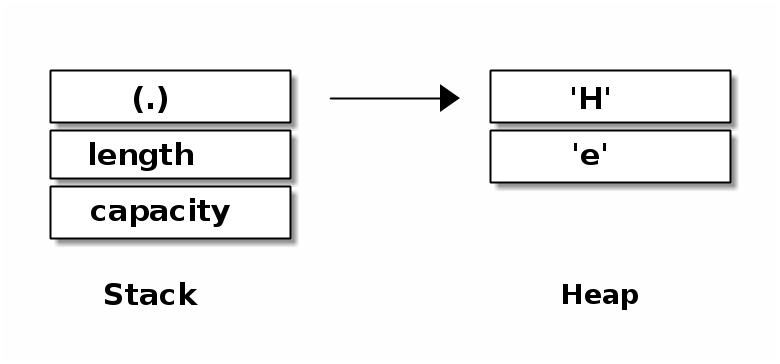
\includegraphics[width=0.55000\textwidth]{images/rust-vec.png}
\caption{Memory layout of a Rust vector}
\end{figure}

In contrast, the memory safe language \emph{Java} enforces a uniform
internal representation of data. In Java a vector has 2 indirections
instead of 1 compared to \emph{Rust} and \emph{C/C++} (cf.
\protect\hyperlink{java-vec}{figure\_title}). As the data could be
represented in a more efficient way in memory, we see that \emph{Java}
does not prioritise the \emph{Zero-Cost-Abstraction} goal.

\begin{figure}[htbp]
\centering
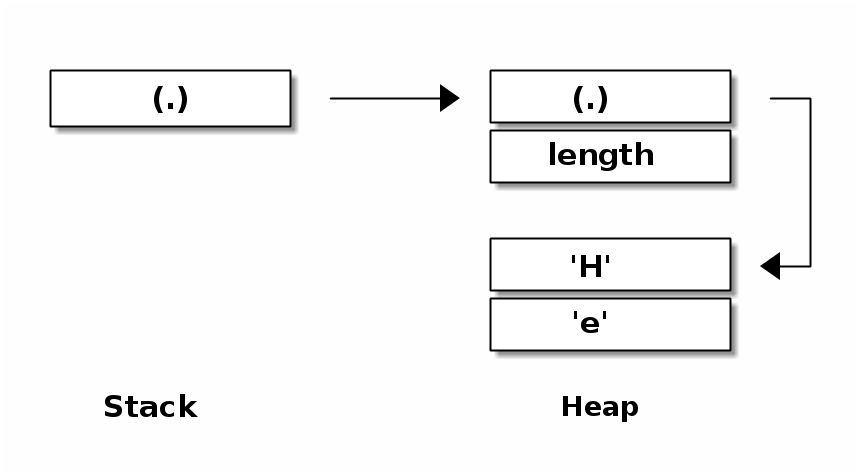
\includegraphics[width=0.60000\textwidth]{images/java-vec.png}
\caption{Memory layout of a Java vector}
\end{figure}

\subsection{Recommendations for novice Rust
programmers}\label{_recommendations_for_novice_rust_programmers}

This chapter introduces two fields of Rust programming that I struggled
with at the beginning. Even when the code does not explicitly annotate
lifetimes and does not use dynamic dispatching, the underlying concepts
are vital for the understanding of Rust's error messages.

\subsubsection{Borrow scope extension}\label{_borrow_scope_extension}

My recommendation for novice programmers is to take the time to
understand Rust's confusing concept of \emph{lifetimes} in detail before
starting a bigger project. In some cases the borrow-scope is not obvious
to see. For example, a second borrower can extend the initial borrow
scope. Liao {[}\protect\hyperlink{liao2014}{14}{]} calls the phenomena
``borrow scope extension''.

\textbf{Borrow cope extension, source code.}

\begin{Shaded}
\begin{Highlighting}[]
\KeywordTok{struct} \NormalTok{Foo \{}
    \NormalTok{f: }\DataTypeTok{Box}\NormalTok{<}\DataTypeTok{isize}\NormalTok{>,}
\NormalTok{\}}

\KeywordTok{fn} \NormalTok{main() \{}
    \KeywordTok{let} \KeywordTok{mut} \NormalTok{a = Foo \{ f: }\DataTypeTok{Box}\NormalTok{::new(}\DecValTok{0}\NormalTok{) \};}
    \KeywordTok{let} \NormalTok{y: &Foo;}
    \KeywordTok{if} \ConstantTok{false} \NormalTok{\{}
        \CommentTok{// borrow}
        \KeywordTok{let} \NormalTok{x = &a; }\CommentTok{// share the borrow with new borrower y,}
                    \CommentTok{// hence extend the borrow scope}
        \NormalTok{y = x;}
    \NormalTok{\}}
    \CommentTok{// error: cannot assign to `a.f` because it is borrowed}
    \NormalTok{a.f = }\DataTypeTok{Box}\NormalTok{::new(}\DecValTok{1}\NormalTok{);}
\NormalTok{\}}
\end{Highlighting}
\end{Shaded}

The following error message only shows the initial borrower whose scope
ends in line 13. The actual problem is caused by line 12 \texttt{y=x}
which extends the initial borrow scope.

\textbf{Borrow scope extension, error message.}

error{[}E0506{]}: cannot assign to `a.f` because it is borrowed
-\/-\textgreater{} \textless{}anon\textgreater{}:15:5 \textbar{} 10
\textbar{} let x = \&a; \textbar{} - borrow of `a.f` occurs here ... 15
\textbar{} a.f = Box::new(1); \textbar{}
\^{}\^{}\^{}\^{}\^{}\^{}\^{}\^{}\^{}\^{}\^{}\^{}\^{}\^{}\^{}\^{}\^{}
assignment to borrowed `a.f` occurs here

To reason about borrows and lifetimes Liao
{[}\protect\hyperlink{liao2014}{14}{]} introduces the following lifetime
scheme, which I find very useful in general. The brackets and va­ria­ble
names refer to the above source code.

\textbf{Borrow scope extension, lifetime scheme.}

\{ a \{ x y \} * \} resource a
\textbar{}\_\_\_\_\_\_\_\_\_\_\_\textbar{} borrower x
\textbar{}\_\_\_\textbar{} x = \&a borrower y
\textbar{}\_\_\_\_\_\textbar{} y = x borrow scope
\textbar{}=======\textbar{} mutate a.f \textbar{} error

\subsubsection{Structure as a borrower}\label{_structure_as_a_borrower}

\emph{Stringext's} two main structures \texttt{Mission} and
\texttt{Finding} are extensively borrowed throuout the source code. When
a structure holds a reference the type-system has to make sure that the
object it points to lives at least as as long as the structure itself.
The following source code shows an example.

\textbf{structure as a borrower, source code.}

\begin{Shaded}
\begin{Highlighting}[]
\KeywordTok{struct} \NormalTok{Foo \{}
    \NormalTok{f: }\DataTypeTok{Box}\NormalTok{<}\DataTypeTok{usize}\NormalTok{>,}
\NormalTok{\}}

\KeywordTok{struct} \NormalTok{Link<}\OtherTok{'a}\NormalTok{> \{}
    \NormalTok{link: &}\OtherTok{'a} \NormalTok{Foo,}
\NormalTok{\}}

\KeywordTok{fn} \NormalTok{main() \{}
    \KeywordTok{let} \NormalTok{a = Foo \{ f: }\DataTypeTok{Box}\NormalTok{::new( }\DecValTok{0} \NormalTok{)\};}
    \KeywordTok{let} \KeywordTok{mut} \NormalTok{x = Link \{ link: &a \};}
    \KeywordTok{if} \ConstantTok{false} \NormalTok{\{}
        \KeywordTok{let} \NormalTok{b = Foo \{ f: }\DataTypeTok{Box}\NormalTok{::new( }\DecValTok{1} \NormalTok{)\};}
        \NormalTok{x.link = &b; }\CommentTok{//error: `b` does not live long enough}
    \NormalTok{\}}
\NormalTok{\}}
\end{Highlighting}
\end{Shaded}

\textbf{Structure as a borrower, error message.}

error: `b` does not live long enough -\/-\textgreater{}
src/main.rs:16:19 \textbar{} 16 \textbar{} x.link = \&b; \textbar{} \^{}
does not live long enough 17 \textbar{} \} \textbar{} - borrowed value
only lives until here 18 \textbar{} \} \textbar{} - borrowed value needs
to live until here

In the above example, the borrower \texttt{x} is borrowing \texttt{a}.
The borrow scope ends at the end of the main block. The commented line
\texttt{x.link\ =\ \&b;} tries to borrow \texttt{b} instead and fails,
because \texttt{b} must live at least as long as \texttt{x}! The
following lifetime scheme illustrates the lifetime dependencies.

\textbf{Structure as a borrower, lifetime scheme.}

\{ a x \{ b * \} \} resource a
\textbar{}\_\_\_\_\_\_\_\_\_\_\_\textbar{} resource b
\textbar{}\_\_\_\textbar{} borrower x
\textbar{}\_\_\_\_\_\_\_\_\_\textbar{} x.link = \&a borrower x
\textbar{}\_\textbar{} x.link = \&b ERROR! borrow scope x
\textbar{}=========\textbar{} b should live at least ¦.....¦

\hypertarget{dev-process}{\section{Software development process and
testing}\label{dev-process}}

The nature and appropriateness of the software development process
impinges on the quality of the resulting software product. For the
development of \emph{Strings­ext} the \emph{test driven development}
methodology was used. This chapter describes the reasons for this
decision and reports on the experience.

\subsection{Risk management}\label{_risk_management}

Based on the functional requirements described in the
\protect\hyperlink{_specifications}{???} and especially in the
\protect\hyperlink{req-concurrent}{section\_title}, the
\protect\hyperlink{req-batch-processing}{section\_title} and the
\protect\hyperlink{req-merge-findings}{section\_title} the algorithm of
the data-flow was defined (cf.
\protect\hyperlink{_scanner_algorithm}{section\_title}).

Once a todo-list was established, \emph{Strings­ext's} core functions
were identified and ordered by risk: What would be the impact on the
whole project if the implementation of a certain function turns out to
be impossible or difficult to realise in the Rust?

Specifically, sorted after risk:

\begin{enumerate}
\def\labelenumi{\arabic{enumi}.}
\item
  \protect\hyperlink{decoder}{section\_title},
\item
  \protect\hyperlink{_concurrency}{section\_title},
\item
  \protect\hyperlink{_polymorphic_io}{section\_title},
\item
  \protect\hyperlink{_merging_vectors}{section\_title},
\item
  \protect\hyperlink{filter}{section\_title}.
\end{enumerate}

For every core function alternative technical solutions were suggested,
implemented, tested and evaluated (cf.
\protect\hyperlink{_analysis_and_design}{???}). This approach allowed at
an early assurance that Rust provides abstractions and solutions for
each of the core functions. It needs to be emphasized that the above
isolated partial solutions do not reveal any indications about their
intercompatibility or temporal behaviour. This risk is addressed in the
next step.

\subsection{Prototype}\label{_prototype}

Regarding the above core functions the encoder library presented the
highest risk. Was its low level interface suitable for the intended
purpose? Was it fast enough? In order to answer these questions a first
prototype with very little functionality was built. The first prototype
showed as proof of concept, that the library meets the expectations.

\hypertarget{_test_driven_development}{\subsection{Test Driven
Development}\label{_test_driven_development}}

From this point on, the actual development of \emph{Strings­ext} was
launched. To meet the high demands in reliability and correctness it had
been developed using the \emph{Test Driven Development} (TDD) method
suggested by Beck {[}\protect\hyperlink{beck2003}{15}{]}.

\subsubsection{Writing tests}\label{_writing_tests}

In conventional software development models, test are written after the
design and implementation phase. In \emph{Test Driven Development} this
order is inverted: every new feature begins with writing a unit test or
modifying an existing one.

Unit tests are isolation tests. They verify one piece of functionality
only and have no dependencies on other test or on the order the tests
are executed. They should not rely on external components such as data
from filesystems, pipes, networks or databases. These external
components have to be simulated by the test-code. The setting-up of the
test environment code is often referred as \emph{test fixture}. A
\emph{test case} is a set of input data and parameters for the
to-be-tested code or function. Once the to-be-tested code is executed,
the result is compared with the expected result. The expected result
must be included in the test case and their relationship should be as
apparent as possible {[}\protect\hyperlink{beck2003}{15 p.~130}{]}.

Rust has an integrated advanced support for unit testing. Here an
example {[}\protect\hyperlink{rustprogramminglanguage2016}{16}{]}:

\textbf{Rust's Unit-Test feature.}

\begin{Shaded}
\begin{Highlighting}[]
\KeywordTok{pub} \KeywordTok{fn} \NormalTok{add_two(a: }\DataTypeTok{i32}\NormalTok{) -> }\DataTypeTok{i32} \NormalTok{\{}
    \NormalTok{a + }\DecValTok{2}
\NormalTok{\}}

\AttributeTok{#[}\NormalTok{test}\AttributeTok{]}
\KeywordTok{fn} \NormalTok{it_works() \{}
    \PreprocessorTok{assert_eq!}\NormalTok{(}\DecValTok{4}\NormalTok{, add_two(}\DecValTok{2}\NormalTok{));}
\NormalTok{\}}
\end{Highlighting}
\end{Shaded}

The test-code in the \protect\hyperlink{unit-test}{formalpara\_title} is
labelled with the compiler directive \texttt{\#{[}test{]}}. This code is
compiled only when Rust's compiler is invoked with \texttt{cargo\ test}.

The test-function \texttt{it\_works()} calls the to-be-tested code
function \texttt{add\_two()} with the test case \texttt{2}. The
assertion macro \texttt{assert\_eq!()} compares the expected result
\texttt{4} with the result of the to-be-tested code and breaks the
test-run in case of failure.

\hypertarget{_development_cycle}{\subsubsection{Development
cycle}\label{_development_cycle}}

Beck {[}\protect\hyperlink{beck2003}{15 p.~9}{]} defines the development
cycle is as follows:

\begin{enumerate}
\def\labelenumi{\arabic{enumi}.}
\item
  Add a little test.

  ``Write a little test that doesn't work, and perhaps doesn't even
  compile at first.''
\item
  Run all tests and fail (\emph{Red}-state).
\item
  Make a little change.

  ``Make the test work quickly, committing whatever sins necessary in
  the process.'' Do not write code that the test does not check.
\item
  Run the tests and succeed (\emph{Green}-state).
\item
  Refactor to remove duplication (\emph{Refactored}-state).
\item
  Commit in your versioning system \footnote{The commit stage is not
    part of the original process, but added here for completeness.} .
\end{enumerate}

Beck {[}\protect\hyperlink{beck2003}{15 p.~11}{]} gives the following
guidelines on how to execute the above steps:

\begin{quote}
\begin{enumerate}
\def\labelenumi{\arabic{enumi}.}
\item
  Write a test. Think about how you would like the operation in your
  mind to appear in your code. You are writing a story. Invent the
  interface you wish you had. Include all the elements in the story that
  you imagine will be necessary to calculate the right answers.
\item
  Make it run. Quickly getting that bar to go to green dominates
  everything else. If a clean, simple solution is obvious, then type it
  in. If the clean, simple solution is obvious but it will take you a
  minute, then make a note of it and get back to the main problem, which
  is getting the bar green in se­conds. This shift in aesthetics is hard
  for some experienced software engineers. They only know how to follow
  the rules of good engineering. Quick green excuses all sins. But only
  for a moment.
\item
  Make it right. Now the system is behaving, put the sinful ways of the
  recent past behind you. Step back onto the straight and narrow path of
  software righteousness. Remove the duplication that you have
  introduced and get to green {[}sic: should be refactored{]} quickly.
\end{enumerate}

The goal is clean code that works {[}\ldots{}​{]}. First we'll solve the
``that works'' part of the problem. Then we'll solve the ``clean code''
part. This is the opposite of architecture-driven development, where you
solve ``clean code'' first, then scramble around trying to integrate
into the design the things you learn as you solve the ``that works''
problem.

---  The general Test Driven Development cycle K. Beck
\end{quote}

\subsubsection{Evaluation and
conclusion}\label{_evaluation_and_conclusion}

It was my first programming experience with \emph{Test Driven
Development} and it took me some time to develop the discipline to
always start coding by writing a test and always observing the 6 stages
of the development cycle. With the new system launched, it soon became
clear what level of efficiency gains could be achieved. Concerning the
\emph{Test Driven Development Cycle} I observed the following:

\begin{description}
\item[From Red-state to Green state]
Making the test fail first and check weather it succeeds after changing
the code, validates the test itself! It proves not only that the new
code implements the new feature correctly, \emph{it also proves that the
test is observing the right functionality.}
\item[From Green-state to Refactored state]
At the beginning I was very sceptical about the ``Make the test work
quickly, committing whatever sins necessary in the process'' suggestion.
Wouldn't it be more economic to write clean code right away? After some
experience I fully agree with the above approach: Very often the
solution is found only after several attempts. Maybe I need a library
function that does not work the way I expected? Maybe I need a language
construct I use for the first time? Finding a solution is creative
process, that will work the best when the programmer sets himself
(temporarily) free from coding conventions. Furthermore, the trial and
error process is more time-economic when refactoring occurs only at the
end of the process. Separating the ``solution finding'' (go into green)
from ``making it right and beautiful'' (refactoring) helps to focus on
what's essential.
\end{description}

Critics of this method argue, that the development process is not
structured enough and the project manager has very little control over
it. It surely depends on the project, but in the present setting the
balance between forward planning and creative freedom was just right.
Moreover, the structuring effect of writing tests in the first place
should not be underestimated. In order to design a test the programmer
must necessarily address the functional requirements before writing the
production code itself. Writing tests also supports code documentation:
the testing code shows in an isolated environment how to interface with
the to-be-tested code. This is very helpful when you need to understand
someone else's code, especially in case of a more complex low level API.
Reading the testing code together with the to be tested code gives you
an idea about the minimum environment a piece of code requires. This way
the testing code supports and completes the \emph{Rustdoc}
in-code-documentation.

\subsection{Documentation}\label{_documentation}

Documentation is an important part of any software project. Rust
projects and APIs are documented by annotating the source code with
special comment-tags
\texttt{\textbackslash{}\textbackslash{}\textbackslash{}} and
\texttt{\textbackslash{}\textbackslash{}!}. Annotations are usually
placed just before the line it refers to. Documentation comments are
written in Markdown. The Rust distribution includes a tool,
\emph{Rustdoc}, that generates the documentation. \emph{Rustdoc}'s
consists of linked html pages, similar to \emph{Javadoc}. The
\emph{Strings­ext} project makes extensive use of \emph{Rust}'s
documentation feature.

The user manual is written in \emph{reStructuredText} format and
compiled to a man-page with \emph{Docutils} (cf.
\protect\hyperlink{stringsext-s-manual-page}{table\_title}).

\hypertarget{_analysis_and_design}{\section{Analysis and
Design}\label{_analysis_and_design}}

This chapter discusses technical solutions complying with the
specifications defined in the \protect\hyperlink{_specifications}{???}
and their implementation in Rust.

\hypertarget{_concurrency}{\subsection{Concurrency}\label{_concurrency}}

The \protect\hyperlink{data-processing-and-threads}{figure\_title} shows
the data flow in \emph{Strings­ext}. All \emph{scanner} instances as
well as the \emph{merger-printer} are designed as threads. Rust uses
OS-level threads and its type and ownership model guarantees the absence
of data races, which are defined as:

\begin{itemize}
\item
  two or more threads in a single process access the same memory
  location concurrently, and
\item
  at least one of the accesses is for writing, and
\item
  the threads are not using any exclusive locks to control their
  accesses to that memory.
\end{itemize}

Rust supports by default two models of inter-thread communication:

\begin{itemize}
\item
  shared memory \footnote{Rust inherits C11's memory model for atomics}
  and
\item
  message channels.
\end{itemize}

\begin{quote}
To communicate between different concurrent parts of the codebase, there
are two marker traits in the type system: ``Send'' and ``Sync''. A type
that is ``Send'' can be transferred between threads. A type that is
``Sync'' can be shared between threads.

Thanks to the type and ownership system, Rust allows safe shared mutable
state. In most programming languages, shared mutable state is the root
of all evil. In Rust, the compiler enforces some rules that prevent data
races from occurring.

The alternative to shared memory are channels. A channel can be used
like a Unix pipe. It has two ends, a sending and a receiving end. Types
that are ``Send'' can be sent through the pipe
{[}\protect\hyperlink{bargen2016}{17}{]}.
\end{quote}

\emph{stringsext} imports the crate ``scoped\_threadpool'' used to
distribute the \emph{shared-memory} \texttt{input\_slice} to its
scanner-threads. Once a scanner has accomplished its mission, it sends
its result through a dedicated \emph{message channel} to the
\emph{merger-printer}-thread. The following code extract illustrates the
implementation:

\textbf{Inter-thread data exchange.}

\begin{Shaded}
\begin{Highlighting}[]
\NormalTok{pool.scoped(|scope| \{ }
    \KeywordTok{for} \NormalTok{mission }\KeywordTok{in} \NormalTok{missions.iter_mut() \{  }
        \KeywordTok{let} \NormalTok{tx = tx.clone();  }
        \NormalTok{scope.execute(}\KeywordTok{move} \NormalTok{|| \{  }
            \KeywordTok{let} \NormalTok{m = Scanner::scan_window (}
                            \NormalTok{&}\KeywordTok{mut} \NormalTok{mission.offset, }
                            \NormalTok{mission.encoding,}
                            \NormalTok{mission.filter_control_chars,}
                            \NormalTok{byte_counter,}
                            \NormalTok{input_slice ); }

             \NormalTok{mission.offset = }\KeywordTok{if} \NormalTok{mission.offset >= WIN_STEP \{ }
                 \NormalTok{mission.offset - WIN_STEP}
             \NormalTok{\} }\KeywordTok{else} \NormalTok{\{}
                 \DecValTok{0}
             \NormalTok{\};}

            \KeywordTok{match} \NormalTok{tx.send(m) \{ }
                 \ConstantTok{Ok}\NormalTok{(_) => \{\},}
                 \ConstantTok{Err}\NormalTok{(_) => \{ }\PreprocessorTok{panic!}\NormalTok{(}\StringTok{"Can not send FindingCollection:"}\NormalTok{); \},}
             \NormalTok{\};}
        \NormalTok{\});}
    \NormalTok{\}}
\NormalTok{\});}
\end{Highlighting}
\end{Shaded}

\begin{itemize}
\item
  Pool with sleeping threads ready to receive a mission.
\item
  Every thread has a context \texttt{mission} with its own variables it
  can read and write.
\item
  Every thread gets a dedicated result-sending-channel.
\item
  In a \texttt{scoped\_treadpool} every thread has read access its
  parent's stack.
\item
  Note that \texttt{Scanner::scan\_window()} is stateless!
\item
  Its output is: \texttt{m}, the result as \texttt{FindingCollection}
  and \texttt{mission.offset} which is pointing to the byte where the
  scanner has stopped.
\item
  The parent's stack access allows threads to read the
  \texttt{input\_slice} concurrently.
\item
  Prepare \texttt{mission.offset} for the next iteration: Update
  \texttt{mission.offset} to indicate the position where the next
  iteration should resume the work.
\item
  Send the result to the \emph{merger-printer}.
\end{itemize}

\begin{figure}[htbp]
\centering
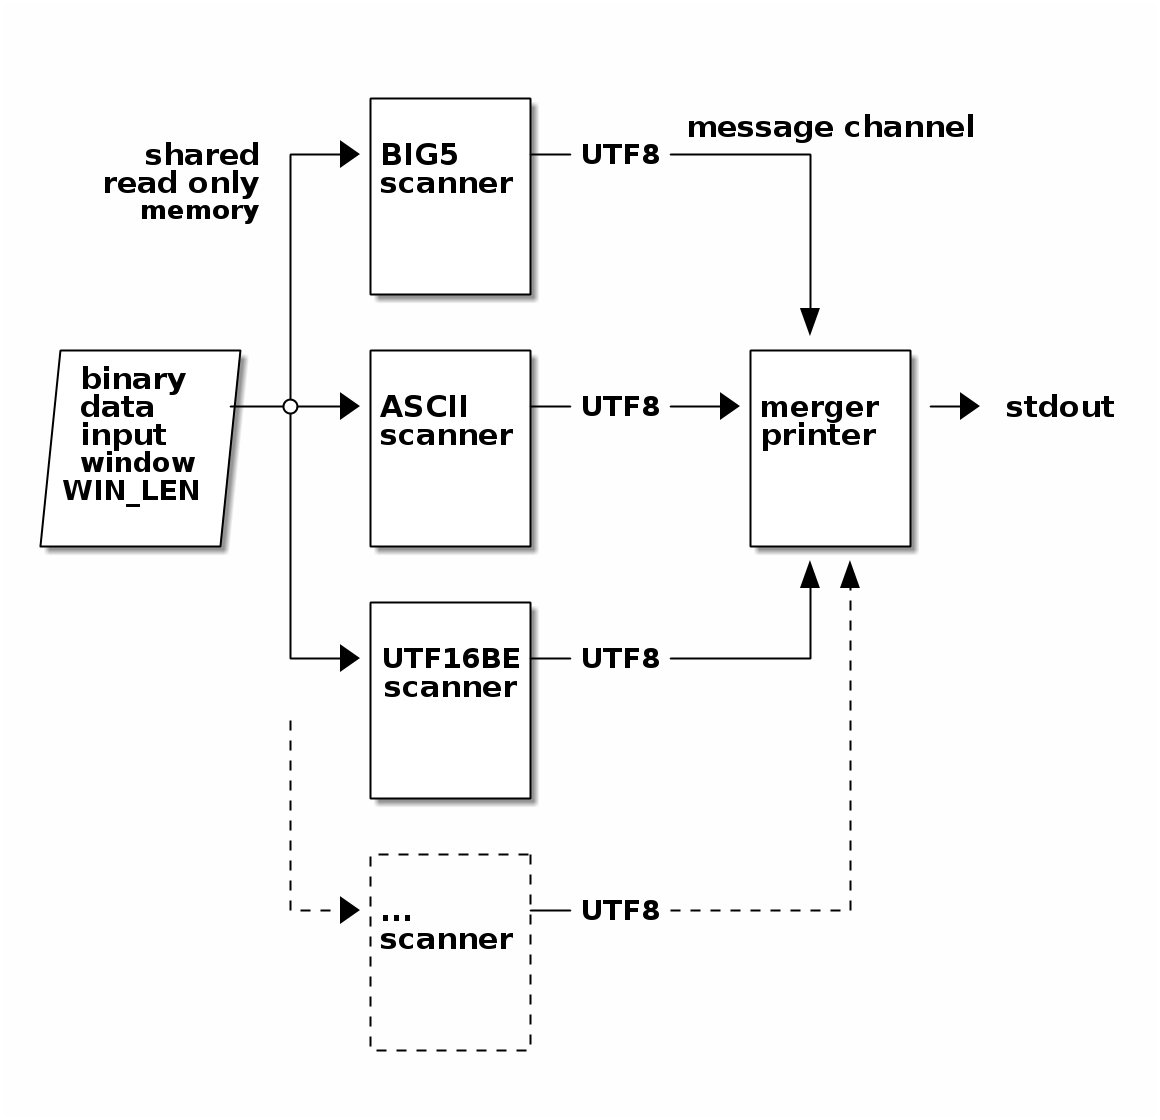
\includegraphics[width=0.80000\textwidth]{images/data-processing-and-thread.png.png}
\caption{Data processing and threads}
\end{figure}

\subsection{Reproducible output}\label{_reproducible_output}

Concurrent computing gives no guarantee in which order partial-output is
available. With regard to \emph{Strings­ext} this means that the order
in which the different scanners report their results, depend on racing
conditions that are not predictable. In order to illustrate this
phenomenon, the
\protect\hyperlink{non-reproducible-output}{figure\_title} shows the
merged output of \emph{Strings­ext}. It is not surprising that for
example at position \texttt{47} and \texttt{c47} the scanners
\emph{ASCII} and \emph{UTF-8} find strings at the same location since
the ASCII-encoding is a subset of the UTF-8 encoding. Whilst at position
\texttt{47} the output of the UTF-8 scanner is first listed, at position
\texttt{c47} the output of the ASCII-scanner is printed first! Even
though the output of \emph{Strings­ext} is always correct, the order in
which the results are presented changes unpredictably!

\begin{figure}[htbp]
\centering
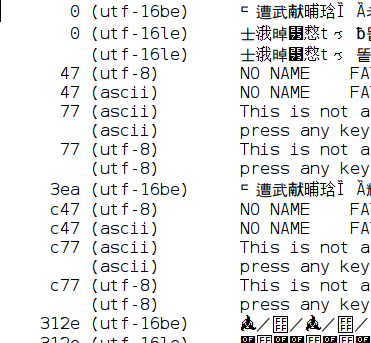
\includegraphics[width=0.40000\textwidth]{images/non-reproducible-output.png}
\caption{Non reproducible output}
\end{figure}

\begin{quote}
\textbf{Important}

An important requirement for forensic tools is \emph{reproducibility}
meaning that the same input-data always produces bit-identical
output-data.
\end{quote}

The retained solution is to extend the sort by criteria which is used by
the merger thread to order the findings. Now it proceeds as follows:
first it sorts by the offset of the finding and then by the encoder name
that has reported the finding. The
\protect\hyperlink{reproducible-output}{figure\_title} shows the result.
Please note that for all identical positions the ASCII-scanner result is
always listed first.

\begin{figure}[htbp]
\centering
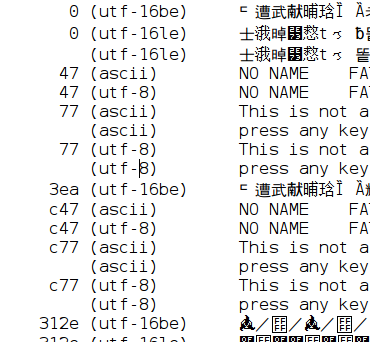
\includegraphics[width=0.40000\textwidth]{images/reproducible-output.png}
\caption{Reproducible output}
\end{figure}

\hypertarget{_scanner_algorithm}{\subsection{Scanner
Algorithm}\label{_scanner_algorithm}}

The input data is processed in batches chunk by chunk. Each chunk is
browsed in parallel by several ``scanner'' threads. This section
describes the algorithm:

\begin{enumerate}
\def\labelenumi{\arabic{enumi}.}
\item
  A \emph{scanner} is a thread with an individual search
  \texttt{Mission} defined by the \emph{encoding} it searches for.
\item
  The input data is divided into consecutive overlapping memory chunks.
  A chunk is a couple of 4KB memory pages, \texttt{WIN\_LEN} bytes in
  size.
\item
  Scanners wait in pause state until they receive a pointer to a memory
  chunk with a dedicated search \texttt{Mission}.
\item
  All scanner-threads search simultaneously in one memory chunk only.
  This avoids that the threads drift to far apart.
\item
  Every scanner thread searches its encoding consecutively byte by byte
  from lower to higher memory.
\item
  When a scanner finds a valid string, it encodes it into a UTF-8 copy,
  called hereafter ``finding''. Valid strings are composed of control
  characters and graphical characters.
\item
  Before storing a finding in \texttt{Finding} object, the above valid
  string is split into one or several graphical strings. Hereby all
  control characters are omitted. The graphical strings are then
  concatenated and the result is stored in a \texttt{Finding} object. A
  \texttt{Finding}-object also carries the memory location (offset) of
  the finding and a pointer describing the search mission. Goto 5.
\item
  A scanner stops when it passes the upper border \texttt{WIN\_STEP} of
  the current memory chunk.
\item
  The scanner stores its \texttt{Finding}-objects in a vector referred
  as \texttt{Findings}. The vector is ascending in memory location.
\item
  Every scanner sends its \texttt{Findings} to the
  \emph{merger-printer-thread}. In order to resume later, it updates a
  marker in its \texttt{Mission}-object pointing to the exact byte where
  it has stopped scanning. Besides this marker, the scanner is
  \emph{stateless}. Finally, the scanner pauses and waits for the next
  memory chunk and mission.
\item
  After all scanners have finished their search in the current chunk,
  the \emph{merger-printer-thread} receives the \texttt{Findings} and
  collects them in a vector.
\item
  The \emph{merger-printer-thread} merges all \texttt{Findings} from all
  threads into one timeline and prints the formatted result through the
  output channel.
\item
  In order to prepare the next iteration, pointers in the
  \texttt{Mission}-objects are set to beginning of the next chunk. Every
  scanner resumes exactly where it stopped before.
\item
  Goto 3.
\item
  Repeat until the last chunk is reached.
\end{enumerate}

\subsection{Memory layout}\label{_memory_layout}

The above algorithm splits the search field into overlapping memory
chunks called \texttt{WIN\_LEN}. Every chunk is also split into 3
fields: \texttt{WIN\_STEP}, \texttt{FINISH\_STR\_BUF} and
\texttt{UTF8\_LEN\_MAX}. This section explains how the algorithm
operates on these fields.

\texttt{WIN\_LEN} is the length of the memory chunk in which strings are
searched in parallel.

\textbf{Memory map.}

\begin{verbatim}
|<WIN_STEP1 -------------->|<WIN_STEP2 --------------->|<WIN_STEP3 -----
                           |<WIN_OVERLAP1>|            |<WIN_OVERLAP2>|
|<WIN_LEN1  ---------------------------- >|
                           |<WIN_LEN2 ------------------------------->|
\end{verbatim}

As shown above, \texttt{WIN\_LEN} defines an overlapping window that
advances \texttt{WIN\_STEP} bytes each iteration.

\texttt{WIN\_LEN\ =\ WIN\_STEP\ +\ WIN\_OVERLAP} is the size of the
memory chunk that is processed during one iteration. A string is only
found when it starts within the \texttt{WIN\_STEP} interval. The
remaining bytes can reach into \texttt{WIN\_OVERLAP} or even beyond
\texttt{WIN\_LEN}. In the latter case the string is split.

\textbf{Constant definition in source code.}

\begin{Shaded}
\begin{Highlighting}[]
   \KeywordTok{pub} \KeywordTok{const} \NormalTok{WIN_LEN: }\DataTypeTok{usize} \NormalTok{= WIN_STEP + WIN_OVERLAP;}
\end{Highlighting}
\end{Shaded}

\texttt{WIN\_OVERLAP} is the overlapping fragment of the window. The
overlapping fragment is used to read some bytes ahead when the string is
not finished. \texttt{WIN\_OVERLAP} is subject to certain conditions:
For example the overlapping part must be smaller than
\texttt{WIN\_STEP}. Furthermore, the size of
\texttt{FINISH\_STR\_BUF\ =\ WIN\_OVERLAP\ -\ UTF8\_LEN\_MAX} determines
the number of bytes at the beginning of a string that are guaranteed not
to be spit.

This size matters because the scanner counts the length of its findings.
If a string is too short (\textless{} \texttt{ARG.flag\_bytes}), it will
be skipped. To avoid that a string with the required size gets too short
because of splitting, we claim the following condition:

\textbf{Constraint.}

\begin{verbatim}
 1 <=  FLAG_BYTES_MAX <=  FINISH_STR_BUF
\end{verbatim}

In practice we chose for \texttt{FINISH\_STR\_BUF} a bigger size than
the minimum to avoid splitting of strings as much as possible. Please
refer to the test function \texttt{test\_constants()} for more details
about constraints on constants. The test checks all the necessary
conditions on constants to guarantee the correct functioning of the
program.

\textbf{Constant definition in source code.}

\begin{Shaded}
\begin{Highlighting}[]
   \KeywordTok{pub} \KeywordTok{const} \NormalTok{FINISH_STR_BUF: }\DataTypeTok{usize} \NormalTok{= }\DecValTok{0x1800}\NormalTok{;}
\end{Highlighting}
\end{Shaded}

The scanner tries to read strings in \texttt{WIN\_LEN} as far as it can.
The first invalid byte indicates the end of a string and the scanner
holds for a moment to store its finding. Then it starts searching
further until the next string is found. Once \texttt{WIN\_OVERLAP} is
entered the search ends and the \texttt{start} variable is updated so
that it now points to \emph{restart-at-invalid} as shown in the next
figure. This way the next iteration can continue at the same place the
previous had stopped.

The next iteration can identify this situation because the
\texttt{start} pointer points into the previous
\texttt{FINISH\_STR\_BUF} interval.

\textbf{Memory map.}

\begin{verbatim}
|<WIN_STEP1 -------------------------->|<FINISH_STR_BUF>|<UTF8_LEN_MAX>|
                                       |<WIN_OVERLAP1>---------------->|
|<WIN_LEN1 ----------------------------------------------------------->|

   <==string==><invalid bytes><=====string===><invalid bytes>
                                              ^
                                              |
                                      `restart-at-invalid`
\end{verbatim}

A special treatment is required when a sting extends slightly beyond
\texttt{WIN\_LEN}. In this case the scanner most likely runs into an
incomplete multi-byte character just before the end of
\texttt{WIN\_LEN}. The cut surface \emph{restart-at-cut} is then
somewhere in the \texttt{UTF8\_LEN\_MAX} interval as the following
figure shows.

The remaining part will be printed later during the next iteration. But
how does the following iteration know if a string had been cut by the
previous iteration? In the next interval the scanner first checks if the
previous scan ended in the \texttt{UTF8\_LEN\_MAX} interval. If yes, we
know the string has been cut and we the remaining bytes at the beginning
of the new interval regardless of their size.

\textbf{Memory map.}

\begin{verbatim}
<...---- WIN_STEP1 ------------->|<FINISH_STR_BUF>|<UTF8_LEN_MAX>|
                                 |<WIN_OVERLAP1>---------------->|
<...---- WIN_LEN1 ---------------------------------------------->|

   <==string==><invalid bytes><====string=============|===========...>
                                                      ^ incomplete
                                                      | valid Multi-
                                                      | byte-Char
                                                      |
                                                `restart-at-cut`
\end{verbatim}

To satisfy all the above constraints \texttt{WIN\_OVERLAP} must satisfy
two conditions concurrently:

\textbf{Constraint.}

\begin{verbatim}
                                   WIN_OVERLAP <= WIN_STEP
FINISH_STR_BUF  + UTF8_LEN_MAX  =  WIN_OVERLAP
\end{verbatim}

\textbf{Constant definition in source code.}

\begin{Shaded}
\begin{Highlighting}[]
   \KeywordTok{pub} \KeywordTok{const} \NormalTok{WIN_OVERLAP: }\DataTypeTok{usize} \NormalTok{= FINISH_STR_BUF + UTF8_LEN_MAX }\KeywordTok{as} \DataTypeTok{usize}\NormalTok{;}
\end{Highlighting}
\end{Shaded}

As Files are accessed through 4KiB memory pages, we choose
\texttt{WIN\_STEP} to be a multiple of 4096 bytes.

\textbf{Constant definition in source code.}

\begin{Shaded}
\begin{Highlighting}[]
   \KeywordTok{pub} \KeywordTok{const} \NormalTok{WIN_STEP: }\DataTypeTok{usize} \NormalTok{= }\DecValTok{0x2000}\NormalTok{; }\CommentTok{// = 2*4096}
\end{Highlighting}
\end{Shaded}

The \texttt{from\_stdin()} function implements its own reader buffer
\texttt{BUF\_LEN} to allow stepping with overlapping windows. The
algorithm requires that \texttt{BUF\_LEN} is greater or equal than
\texttt{WIN\_LEN} (the greater the better the performance).

\textbf{Constraint.}

\begin{verbatim}
     WIN_LEN <= BUF_LEN
\end{verbatim}

Every time \texttt{BUF\_LEN} is full, the last \texttt{WIN\_OVERLAP}
part must be copied from the end to the beginning of \texttt{BUF\_LEN}.
As copying is an expensive operation we choose:

\textbf{Constraint.}

\begin{verbatim}
     BUF_LEN = 4 * WIN_STEP + WIN_OVERLAP
\end{verbatim}

The above reduces the copying to every 4th iteration.

\textbf{Constant definition in source code.}

pub const BUF\_LEN: usize = 4 * WIN\_STEP + WIN\_OVERLAP;

In Unicode the maximum number of bytes a multi-byte-character can occupy
in memory is 6 bytes.

\textbf{Constant definition in source code.}

\begin{Shaded}
\begin{Highlighting}[]
   \KeywordTok{pub} \KeywordTok{const} \NormalTok{UTF8_LEN_MAX: }\DataTypeTok{u8} \NormalTok{= }\DecValTok{6}\NormalTok{;}
\end{Highlighting}
\end{Shaded}

\hypertarget{decoder}{\subsection{Integration with a decoder
library}\label{decoder}}

To meet the requirements defined in the
\protect\hyperlink{character-encoding-support}{section\_title}
\emph{Strings­ext}'s scanners perform a code conversion of their
findings towards UTF-8 (see also
\protect\hyperlink{data-processing-and-threads}{figure\_title}).
Encoding conversion is a very complex matter: the Unicode specification
alone has 1036 pages
{[}\protect\hyperlink{unicodeconsortium2016}{18}{]}! And Unicode is not
the only encoding involved in \emph{Strings­ext}'s data processing.

It will come as no surprise that encoding conversion is related to
numerous vulnerabilities (see the
\protect\hyperlink{security2}{section\_title} for details).

Basically, there are two ways to interface a third party library in
Rust:

\begin{enumerate}
\def\labelenumi{\arabic{enumi}.}
\item
  Writing bindings for a C library using the Foreign Function Interface
  {[}\protect\hyperlink{rustprogramminglanguage2016}{16}{]}.
\item
  Using a native Rust library.
\end{enumerate}

In order to address potential security issues discussed in the
\protect\hyperlink{security2}{section\_title} the second option ``native
Rust library'' had been chosen. \emph{Strings­ext} uses the so called
\emph{rust/encoding} library developed by Seonghoon
{[}\protect\hyperlink{seonghoon2016}{19}{]}.

\emph{rust/encoding} provides encoder and decoder functionality for the
following encodings specified by the WHATWG encoding standard:

\begin{itemize}
\item
  7-bit strict ASCII (ascii)
\item
  UTF-8 (utf-8)
\item
  UTF-16 in little endian (utf-16 or utf-16le)
\item
  UTF-16 in big endian (utf-16be)
\item
  Single byte encodings in according to the WHATWG encoding standard:

  \begin{itemize}
  \item
    IBM code page 866
  \item
    ISO 8859-1 (distinct from Windows code page 1252)
  \item
    ISO 8859-2, ISO 8859-3, ISO 8859-4, ISO 8859-5, ISO 8859-6, ISO
    8859-7, ISO 8859-8, ISO 8859-10, ISO 8859-13, ISO 8859-14, ISO
    8859-15, ISO 8859-16
  \item
    KOI8-R, KOI8-U
  \item
    MacRoman (macintosh), Macintosh Cyrillic encoding (x-mac-cyrillic)
  \item
    Windows code pages 874, 1250, 1251, 1252 (instead of ISO 8859-1),
    1253, 1254 (instead of ISO 8859-9), 1255, 1256, 1257, 1258
  \end{itemize}
\item
  Multi byte encodings according to the WHATWG Encoding standard:

  \begin{itemize}
  \item
    Windows code page 949 (euc-kr, since the strict EUC-KR is hardly
    used)
  \item
    EUC-JP and Windows code page 932 (shift\_jis, since it's the most
    widespread extension to Shift\_JIS)
  \item
    ISO-2022-JP with asymmetric JIS X 0212 support (Note: this is not
    yet up to date to the current standard)
  \item
    GBK
  \item
    GB 18030
  \item
    Big5-2003 with HKSCS-2008 extensions
  \end{itemize}
\item
  Encodings that were originally specified by WHATWG encoding standard:

  \begin{itemize}
  \item
    HZ
  \end{itemize}
\end{itemize}

\hypertarget{filter}{\subsection{Valid string to graphical string
filter}\label{filter}}

The \emph{rust/encoding} library was originally not designed to search
for strings in binary data. Nevertheless, the low level API function
\texttt{decoder.raw\_feed()} returns and decodes chunks of \emph{valid}
strings found in the input stream. Those \emph{valid strings} are then
always re-encoded to UTF-8 and comprise:

\begin{itemize}
\item
  \textbf{Graphical characters} represent a written symbol. When
  printed, toner or ink can be seen on the paper.

  \begin{quote}
  \textbf{Note}

  \emph{GNU-strings} and \emph{Strings­ext} consider SPACE and TAB as
  graphical characters.
  \end{quote}
\item
  \textbf{Control characters} have no visual or spatial representation.
  They control the interpretation or display of text.
\end{itemize}

As the \emph{rust/encoding} library returns \emph{valid} strings and
\emph{Strings­ext} prints by default only \emph{graphical} strings, and
additional filter must be applied:

\textbf{Control character filter.}

\begin{Shaded}
\begin{Highlighting}[]
\KeywordTok{let} \NormalTok{len = $fc.v.last().unwrap().s.len();}
\KeywordTok{let} \KeywordTok{mut} \NormalTok{out = }\DataTypeTok{String}\NormalTok{::with_capacity(len); }
\NormalTok{\{}
    \KeywordTok{let} \KeywordTok{mut} \NormalTok{chunks = (&$fc).v.last().unwrap().s }
        \NormalTok{.split_terminator(|c: }\DataTypeTok{char}\NormalTok{|}
                          \NormalTok{c.is_control()}
                          \NormalTok{&& c != }\CharTok{' '} \NormalTok{&& c !=}\CharTok{'}\SpecialCharTok{\textbackslash{}t}\CharTok{'}
        \NormalTok{)  }
        \NormalTok{.enumerate()}
        \NormalTok{.filter(|&(n,s)| (s.len() >= minsize ) ||  }
                         \NormalTok{((n == }\DecValTok{0}\NormalTok{) && $fc.completes_last_str) }
        \NormalTok{)}
        \NormalTok{.map(|(_, s)| s );}

    \KeywordTok{if} \KeywordTok{let} \ConstantTok{Some}\NormalTok{(first_chunk) = chunks.next() \{ }
        \KeywordTok{if} \NormalTok{!$fc.v.last().unwrap().s.starts_with(&first_chunk) \{ }
            \NormalTok{out.push_str(&CONTROL_REPLACEMENT_STR); }
        \NormalTok{\}}
        \NormalTok{out.push_str(first_chunk);}
        \KeywordTok{for} \NormalTok{chunk }\KeywordTok{in} \NormalTok{chunks \{ }
            \NormalTok{out.push_str(&CONTROL_REPLACEMENT_STR);}
            \NormalTok{out.push_str(chunk);}
        \NormalTok{\}}
    \NormalTok{\}}
\NormalTok{\};}
\end{Highlighting}
\end{Shaded}

\begin{itemize}
\item
  \texttt{out} is the filtered string containing all concatenated
  graphical strings.
\item
  \texttt{(\&\$fc).v.last().unwrap().s} is the \emph{valid input} string
  comprising control and graphical characters.
\item
  Iterator over chunks of graphical strings.
\item
  Filter out too short strings,
\item
  unless they do not complete a cut off string from the previous scanner
  run.
\item
  Read the first graphical string.
\item
  Had there been control characters before it?
\item
  Place a \texttt{CONTROL\_REPLACEMENT\_STR} character. The actually
  inserted character depend on the \texttt{-\/-control-chars}
  command-line option: For \texttt{-\/-control-chars=r} the character
  \texttt{\textbackslash{}u\{fffd\}} is inserted. For
  \texttt{-\/-control-chars=i} the character \texttt{\textbackslash{}n}
  (newline) is inserted.
\item
  Concatenate all the remaining graphical strings and place a
  \texttt{CONTROL\_REPLACEMENT\_STR} in between each.
\end{itemize}

All scanners use the above filter unless the command-line option
\texttt{-\/-control-chars=p} is given. Then the whole valid string is
printed with all its control characters.

The only exception to this occurs for the options
\texttt{-e\ ascii\ -c\ i}. This combination invokes a specially designed
ASCII-graphical-strings-only decoder. This approach made it possible to
generate a bit identical output compared to \emph{GNU-strings} for this
setting.

The option \texttt{-\/-control-chars=r} addresses especially the
requirement defined in the
\protect\hyperlink{req-post-treatment}{section\_title}. All control
characters are replaced by \texttt{\textbackslash{}u\{fffd\}} keeping
the filtered string always in one line. Together with the formatting
option \texttt{-t} the printed lines have the following syntax:

\begin{verbatim}
<offset>'\t('<encoding name>')\t'<graphical string>'\u{fffd}'<graphical...
\end{verbatim}

\hypertarget{_polymorphic_io}{\subsection{Polymorphic
IO}\label{_polymorphic_io}}

\emph{GNU-strings} can read its input from a file, or from a pipe. Both
requires different optimisation strategies. The fastest way to read a
file sequentially is through the \emph{memory mapping} kernel interface.
\emph{danburkert/memmap-rs} is a Rust library for cross-platform
memory-mapped file IO. An interesting feature of \emph{memory mapping}
is that it can map files much larger than the available RAM to a
\emph{virtual address space}. This allows to map the whole file regards
to its size and iterate over it with a sliding window. The following
code extract shows this technique. Note that there is only one call of
the \texttt{Mmap::open()} wrapper occurring outside the loop. This
reduces the overhead caused by the wrapper.

\textbf{Memory mapping the entire file.}

\begin{Shaded}
\begin{Highlighting}[]
\KeywordTok{let} \KeywordTok{mut} \NormalTok{byte_counter: }\DataTypeTok{usize} \NormalTok{= }\DecValTok{0}\NormalTok{;}
\KeywordTok{let} \NormalTok{file = }\PreprocessorTok{try!}\NormalTok{(Mmap::open(file, Protection::Read)); }
\KeywordTok{let} \NormalTok{bytes = }\KeywordTok{unsafe} \NormalTok{\{ file.as_slice() \};}
\KeywordTok{let} \NormalTok{len = bytes.len();}
\KeywordTok{for} \NormalTok{chunk }\KeywordTok{in} \NormalTok{bytes.windows(WIN_LEN).step(WIN_STEP) \{}
    \NormalTok{sc.launch_scanner(&byte_counter, &chunk); }
    \NormalTok{byte_counter += WIN_STEP;}
\NormalTok{\}}
\end{Highlighting}
\end{Shaded}

\begin{itemize}
\item
  Map the whole file contents in virtual address space.
\item
  Launch the scanner threads providing a chunk of memory.
\end{itemize}

An alternative technique consists mapping memory pages sequentially page
by page. The following code shows this approach. Note that the call of
\texttt{Mmap::open\_with\_offset()} happens inside the loop!

\textbf{Memory mapping page by page.}

\begin{Shaded}
\begin{Highlighting}[]
\KeywordTok{let} \NormalTok{len = }\PreprocessorTok{try!}\NormalTok{(file.metadata()).len() }\KeywordTok{as} \DataTypeTok{usize}\NormalTok{;}
\KeywordTok{let} \KeywordTok{mut} \NormalTok{byte_counter: }\DataTypeTok{usize} \NormalTok{= }\DecValTok{0}\NormalTok{;}
\KeywordTok{while} \NormalTok{byte_counter + WIN_LEN <= len \{}
    \KeywordTok{let} \NormalTok{mmap = Mmap::open_with_offset(&file, Protection::Read,  }
                                      \NormalTok{byte_counter,WIN_LEN).unwrap();}
    \KeywordTok{let} \NormalTok{chunk = }\KeywordTok{unsafe} \NormalTok{\{ mmap.as_slice() \};}
    \NormalTok{sc.launch_scanner(&byte_counter, &chunk);  }
    \NormalTok{byte_counter += WIN_STEP;}
\NormalTok{\}}
\end{Highlighting}
\end{Shaded}

\begin{itemize}
\item
  Map a few numbers of memory pages only.
\item
  Pass them to the scanner threads.
\end{itemize}

Tests with big files showed that memory mapping page by page is faster
despite its overhead. One reason is that the other solution does not
launch the scanner right from the start: the operating system reads the
whole data in memory before giving the control back to the calling
program. This does not only consume a lot of memory but also holds back
the scanners when the program starts. This is why the solution
\emph{Memory mapping page by page} was selected: it reads only very few
memory pages into memory and the scanner can start their work much
earlier.

Note that the function \texttt{as\_slice()} is tagged ``unsafe''. It
means that the file-reading operation is only safe as long as no other
process writes that file simultaneously. I consider this requirement to
be met for all use cases of \emph{Strings­ext} and we do not implement
any additional file locking mechanism.

The second operation mode ``reading input from a pipe'' raised another
challenge: None of the standard input readers is able to read by
overlapping chunks. To solve the problem a circular-buffer was
implemented. The following shows an extract of the source code.

\textbf{Circular input buffer.}

\begin{Shaded}
\begin{Highlighting}[]
\KeywordTok{while} \NormalTok{!done \{}
    \CommentTok{// Rotate the buffer if there isn't enough space }
    \KeywordTok{if} \NormalTok{data_start + WIN_LEN > BUF_LEN \{}
        \KeywordTok{let} \NormalTok{(a, b) = buf.split_at_mut(data_start);}
        \KeywordTok{let} \NormalTok{len = data_end - data_start;}
        \NormalTok{a[..len].copy_from_slice(&b[..len]);}
        \NormalTok{data_start = }\DecValTok{0}\NormalTok{;}
        \NormalTok{data_end = len;}
    \NormalTok{\}}
    \CommentTok{// Read from stdin}
    \KeywordTok{while} \NormalTok{data_end < data_start + WIN_LEN \{         }
        \KeywordTok{let} \NormalTok{bytes = }\PreprocessorTok{try!}\NormalTok{(stdin.read(&}\KeywordTok{mut} \NormalTok{buf[data_end..]));}
        \KeywordTok{if} \NormalTok{bytes == }\DecValTok{0} \NormalTok{\{}
            \NormalTok{done = }\ConstantTok{true}\NormalTok{;}
            \KeywordTok{break}\NormalTok{;}
        \NormalTok{\}}
        \KeywordTok{else} \NormalTok{\{data_end += bytes; \}}
    \NormalTok{\}}
    \CommentTok{// Handle data.                                 }
    \KeywordTok{while} \NormalTok{data_start + WIN_LEN <= data_end \{}
        \NormalTok{sc.launch_scanner(&byte_counter,}
                \NormalTok{&buf[data_start..data_start + WIN_LEN]);}
        \NormalTok{data_start += WIN_STEP;}
        \NormalTok{byte_counter += WIN_STEP;}
    \NormalTok{\}}
\NormalTok{\}}
\end{Highlighting}
\end{Shaded}

\begin{itemize}
\item
  Make sure that there is always enough space to receive the next input
  chunk.
\item
  Fill the buffer from \texttt{stdin}.
\item
  Empty the buffer by reading \texttt{WIN\_LEN} bytes.
\end{itemize}

\hypertarget{_merging_vectors}{\subsection{Merging
vectors}\label{_merging_vectors}}

The \emph{merger-printer} thread in the
\protect\hyperlink{data-processing-and-threads}{figure\_title} receives
vectors of \texttt{Findings} from the connected upstream scanners. Every
input vector is sorted by memory offset.

To merge the input vectors two alternative solutions have been
developed.

The first solution is based on a contribution of Jake Goulding, aka
Shepmaster, who posted the following code realising an iterator able to
merge 2 vectors {[}\protect\hyperlink{goulding2015}{20}{]}.

\textbf{Merging iterator for two vectors.}

\begin{Shaded}
\begin{Highlighting}[]
\KeywordTok{use} \NormalTok{std::iter::Peekable;}
\KeywordTok{use} \NormalTok{std::cmp::Ordering;}

\KeywordTok{struct} \NormalTok{MergeAscending<L, R>}
    \KeywordTok{where} \NormalTok{L: }\BuiltInTok{Iterator}\NormalTok{<Item = R::Item>, R: }\BuiltInTok{Iterator}\NormalTok{,}
\NormalTok{\{}
    \NormalTok{left: Peekable<L>,}
    \NormalTok{right: Peekable<R>,}
\NormalTok{\}}

\KeywordTok{impl}\NormalTok{<L, R> MergeAscending<L, R>}
    \KeywordTok{where} \NormalTok{L: }\BuiltInTok{Iterator}\NormalTok{<Item = R::Item>, R: }\BuiltInTok{Iterator}\NormalTok{,}
\NormalTok{\{}
    \KeywordTok{fn} \NormalTok{new(left: L, right: R) -> }\KeywordTok{Self} \NormalTok{\{}
        \NormalTok{MergeAscending \{}
            \NormalTok{left: left.peekable(),}
            \NormalTok{right: right.peekable(),}
        \NormalTok{\}}
    \NormalTok{\}}
\NormalTok{\}}

\KeywordTok{impl}\NormalTok{<L, R> }\BuiltInTok{Iterator} \KeywordTok{for} \NormalTok{MergeAscending<L, R>}
    \KeywordTok{where} \NormalTok{L: }\BuiltInTok{Iterator}\NormalTok{<Item = R::Item>, R: }\BuiltInTok{Iterator}\NormalTok{, L::Item: }\BuiltInTok{Ord}\NormalTok{,}
\NormalTok{\{}
    \KeywordTok{type} \NormalTok{Item = L::Item;}
    \KeywordTok{fn} \NormalTok{next(&}\KeywordTok{mut} \KeywordTok{self}\NormalTok{) -> }\DataTypeTok{Option}\NormalTok{<L::Item> \{}
        \KeywordTok{let} \NormalTok{which = }\KeywordTok{match} \NormalTok{(}\KeywordTok{self}\NormalTok{.left.peek(), }\KeywordTok{self}\NormalTok{.right.peek()) \{}
            \NormalTok{(}\ConstantTok{Some}\NormalTok{(l), }\ConstantTok{Some}\NormalTok{(r)) => }\ConstantTok{Some}\NormalTok{(l.cmp(r)),}
            \NormalTok{(}\ConstantTok{Some}\NormalTok{(_), }\ConstantTok{None}\NormalTok{)    => }\ConstantTok{Some}\NormalTok{(Ordering::Less),}
            \NormalTok{(}\ConstantTok{None}\NormalTok{, }\ConstantTok{Some}\NormalTok{(_))    => }\ConstantTok{Some}\NormalTok{(Ordering::Greater),}
            \NormalTok{(}\ConstantTok{None}\NormalTok{, }\ConstantTok{None}\NormalTok{)       => }\ConstantTok{None}\NormalTok{,}
        \NormalTok{\};}
        \KeywordTok{match} \NormalTok{which \{}
            \ConstantTok{Some}\NormalTok{(Ordering::Less)    => }\KeywordTok{self}\NormalTok{.left.next(),}
            \ConstantTok{Some}\NormalTok{(Ordering::Equal)   => }\KeywordTok{self}\NormalTok{.left.next(),}
            \ConstantTok{Some}\NormalTok{(Ordering::Greater) => }\KeywordTok{self}\NormalTok{.right.next(),}
            \ConstantTok{None}                    \NormalTok{=> }\ConstantTok{None}\NormalTok{,}
        \NormalTok{\}}
    \NormalTok{\}}
\NormalTok{\}}
\end{Highlighting}
\end{Shaded}

The following testing code illustrates how to merge two vectors.

\textbf{Testing code merging iterator for two vectors.}

\begin{Shaded}
\begin{Highlighting}[]
\AttributeTok{#[}\NormalTok{test}\AttributeTok{]}
\KeywordTok{fn} \NormalTok{merge_two_iterators_concrete_types() \{}
    \KeywordTok{let} \NormalTok{left  = [}\DecValTok{1}\NormalTok{, }\DecValTok{3}\NormalTok{, }\DecValTok{5}\NormalTok{, }\DecValTok{7}\NormalTok{, }\DecValTok{9}\NormalTok{];}
    \KeywordTok{let} \NormalTok{right = [}\DecValTok{3}\NormalTok{, }\DecValTok{4}\NormalTok{, }\DecValTok{5}\NormalTok{, }\DecValTok{6}\NormalTok{];}
    \KeywordTok{let} \NormalTok{result: }\DataTypeTok{Vec}\NormalTok{<_> =}
        \NormalTok{MergeAscending::new(left.iter(), right.iter()).collect();}

    \KeywordTok{let} \NormalTok{expected = }\PreprocessorTok{vec!}\NormalTok{[}\DecValTok{1}\NormalTok{, }\DecValTok{3}\NormalTok{, }\DecValTok{3}\NormalTok{, }\DecValTok{4}\NormalTok{, }\DecValTok{5}\NormalTok{, }\DecValTok{5}\NormalTok{, }\DecValTok{6}\NormalTok{, }\DecValTok{7}\NormalTok{, }\DecValTok{9}\NormalTok{];}
    \CommentTok{// result == expected?}
    \PreprocessorTok{assert!}\NormalTok{( result.iter().zip(expected).all(|(&a,b)| a-b == }\DecValTok{0} \NormalTok{)}
    \NormalTok{);}
\NormalTok{\}}
\end{Highlighting}
\end{Shaded}

Jake Goulding's code, as shown above, can only merge two vectors. The
following macro, realised by the author of this present work, extends
the above code by adding successively iterators. The resulting algorithm
to find the next element is basically a linear search. Its complexity is
\texttt{O(N\ *\ k)}, where \texttt{N} is the total length of iterables
and \texttt{k} is the number of iterables.

\textbf{Merging iterator for multiple vectors.}

\begin{Shaded}
\begin{Highlighting}[]
\PreprocessorTok{macro_rules!} \NormalTok{merging_iterator_from \{}
    \NormalTok{($vv: ident) => \{\{}
        \KeywordTok{let} \KeywordTok{mut} \NormalTok{ma: }\DataTypeTok{Box}\NormalTok{<}\BuiltInTok{Iterator}\NormalTok{<Item=_>> =}
                    \DataTypeTok{Box}\NormalTok{::new($vv[}\DecValTok{0}\NormalTok{].iter().map(|&i|i));}
        \KeywordTok{for} \NormalTok{v }\KeywordTok{in} \NormalTok{$vv.iter().skip(}\DecValTok{1}\NormalTok{) \{}
            \NormalTok{ma = }\DataTypeTok{Box}\NormalTok{::new(MergeAscending::new(ma, v.iter().map(|&i|i)));}
        \NormalTok{\};}
        \NormalTok{ma}
    \NormalTok{\}\}}
\NormalTok{\}}
\end{Highlighting}
\end{Shaded}

The following testing code illustrates how to merge 5 vectors.

\textbf{Testing code merging iterator for multiple vectors.}

\begin{Shaded}
\begin{Highlighting}[]
\AttributeTok{#[}\NormalTok{test}\AttributeTok{]}
\KeywordTok{fn} \NormalTok{merge_five_iterators() \{}
    \KeywordTok{let} \NormalTok{vv: }\DataTypeTok{Vec}\NormalTok{<}\DataTypeTok{Vec}\NormalTok{<_>> = }\PreprocessorTok{vec!}\NormalTok{[}
        \PreprocessorTok{vec!}\NormalTok{[}\DecValTok{1}\NormalTok{, }\DecValTok{3}\NormalTok{, }\DecValTok{5}\NormalTok{, }\DecValTok{7}\NormalTok{, }\DecValTok{9}\NormalTok{],}
        \PreprocessorTok{vec!}\NormalTok{[}\DecValTok{3}\NormalTok{, }\DecValTok{4}\NormalTok{, }\DecValTok{6}\NormalTok{, }\DecValTok{7}\NormalTok{],}
        \PreprocessorTok{vec!}\NormalTok{[}\DecValTok{0}\NormalTok{, }\DecValTok{6}\NormalTok{, }\DecValTok{8}\NormalTok{],}
        \PreprocessorTok{vec!}\NormalTok{[}\DecValTok{1}\NormalTok{, }\DecValTok{2}\NormalTok{, }\DecValTok{12}\NormalTok{],}
        \PreprocessorTok{vec!}\NormalTok{[}\DecValTok{10}\NormalTok{]}
    \NormalTok{];}

    \KeywordTok{let} \NormalTok{result: }\DataTypeTok{Vec}\NormalTok{<_> = }\PreprocessorTok{merging_iterator_from!}\NormalTok{(vv).collect::<}\DataTypeTok{Vec}\NormalTok{<_>>();}

    \KeywordTok{let} \NormalTok{expected = }\PreprocessorTok{vec!}\NormalTok{[}\DecValTok{0}\NormalTok{, }\DecValTok{1}\NormalTok{, }\DecValTok{1}\NormalTok{, }\DecValTok{2}\NormalTok{, }\DecValTok{3}\NormalTok{, }\DecValTok{3}\NormalTok{, }\DecValTok{4}\NormalTok{, }\DecValTok{5}\NormalTok{, }\DecValTok{6}\NormalTok{, }\DecValTok{6}\NormalTok{, }\DecValTok{7}\NormalTok{, }\DecValTok{7}\NormalTok{, }\DecValTok{8}\NormalTok{, }\DecValTok{9}\NormalTok{, }\DecValTok{10}\NormalTok{, }\DecValTok{12}\NormalTok{];}
    \CommentTok{// result == expected?}
    \PreprocessorTok{assert!}\NormalTok{( result.iter().zip(expected).all(|(&a,b)| a-b == }\DecValTok{0} \NormalTok{)}
    \NormalTok{);}
\NormalTok{\}}
\end{Highlighting}
\end{Shaded}

For test purposes, the above 4 code samples can be concatenated in one
file.

The benefit of this solution is its simplicity and that it does not
require any external library. Sure, linear search is not the fastest
algorithm, but seeing the little number of vectors we have to merge this
is not necessarily a drawback.

Shortly after I implemented the above solution, the iterator
\texttt{kmerge} was published in the \emph{rust/itertools} library. It
implements the heapsort algorithm. The complexity of the approach is
\texttt{O(N\ *\ log(k))}, where \texttt{N} is the total length of
iterables and \texttt{k} is the number of iterables. Its better
performance, compared to the first solution, is practically negligible
in the present case as number of iterables is relatively small.

The next testing code sample shows how to merge 3 vectors.

\textbf{Testing code kmerge library.}

\begin{Shaded}
\begin{Highlighting}[]
\KeywordTok{extern} \KeywordTok{crate} \NormalTok{itertools;}
\KeywordTok{use} \NormalTok{itertools::free::kmerge;}

\AttributeTok{#[}\NormalTok{test}\AttributeTok{]}
\KeywordTok{fn} \NormalTok{merge_three_iterators() \{}
    \KeywordTok{let} \NormalTok{vv = }\PreprocessorTok{vec!}\NormalTok{[}
        \PreprocessorTok{vec!}\NormalTok{[}\DecValTok{0}\NormalTok{, }\DecValTok{2}\NormalTok{, }\DecValTok{4}\NormalTok{],}
        \PreprocessorTok{vec!}\NormalTok{[}\DecValTok{1}\NormalTok{, }\DecValTok{2}\NormalTok{, }\DecValTok{5}\NormalTok{],}
        \PreprocessorTok{vec!}\NormalTok{[}\DecValTok{3}\NormalTok{, }\DecValTok{7}\NormalTok{]}
    \NormalTok{];}

    \KeywordTok{let} \NormalTok{result = kmerge(&vv).collect::<}\DataTypeTok{Vec}\NormalTok{<_>>();}

    \KeywordTok{let} \NormalTok{expected = }\PreprocessorTok{vec!}\NormalTok{[}\DecValTok{0}\NormalTok{, }\DecValTok{1}\NormalTok{, }\DecValTok{2}\NormalTok{, }\DecValTok{2}\NormalTok{, }\DecValTok{3}\NormalTok{, }\DecValTok{4}\NormalTok{, }\DecValTok{5}\NormalTok{, }\DecValTok{7}\NormalTok{];}

    \CommentTok{// result == expected?}
    \PreprocessorTok{assert_eq!}\NormalTok{(result.len(),expected.len());}
    \PreprocessorTok{assert!}\NormalTok{( result.iter().zip(expected).all(|(&a,b)| a-b == }\DecValTok{0} \NormalTok{)}
    \NormalTok{);}
\NormalTok{\}}
\end{Highlighting}
\end{Shaded}

For \emph{Strings­ext} I finally chose the second solution with
\texttt{kmerge}. Its slightly better performance is surely desirable,
but most of all it was my intention of keeping \emph{Strings­ext}'s code
base as small as possible that led to the decision using the external
\texttt{kmerge}-function of the \emph{rust/itertools} library.

\section{Strings­ext's usage and product
evaluation}\label{_strings_ext_s_usage_and_product_evaluation}

The initial motivation for developing \emph{Strings­ext} were the
various shortcomings of \emph{GNU-strings} especially when it comes to
handle international cha­rac­ter encodings. Does \emph{Strings­ext}
support foreign scripts better? Is it as fast?

\subsection{Test case 2 - international character
encodings}\label{test-case-stringsext}

To evaluate \emph{Strings­ext}'s capabilities to handle international
scripts with Unicode we chose the same text file as input we used with
\emph{GNU-strings} in the
\protect\hyperlink{test-case-strings}{section\_title}:

\begin{figure}[htbp]
\centering
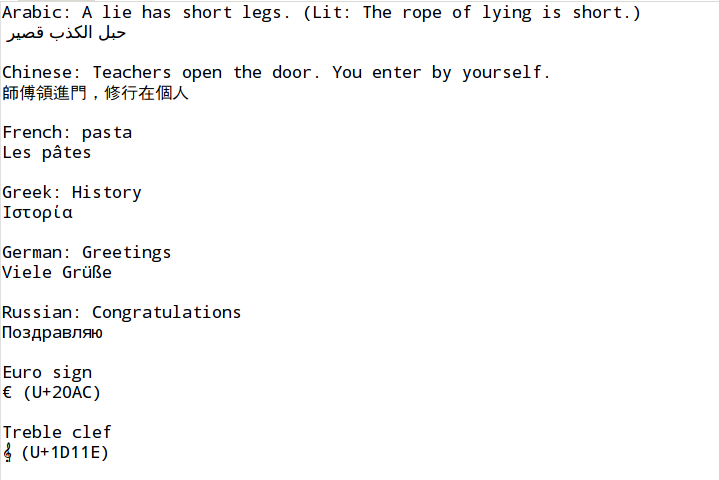
\includegraphics[width=0.80000\textwidth]{images/orig.png}
\caption{Unicode test-file: orig.txt}
\end{figure}

The following bash-script automates the test case generation: To provide
a copy of the test file in UTF-8, UTF-16be, UTF-16le, UTF-32be and
UTF-32le encodings the Unix tool \texttt{iconv} is used.

The second part of the script feeds the generated copies one by one into
\emph{Strings­ext}. The options
\texttt{-e\ ascii\ -e\ utf-8\ -e\ utf-16be\ -e\ utf-16le} instruct
\emph{Strings­ext} to search for the following encodings: ASCII, UTF-8,
UTF-16be, UTF-16le. Please refer to
\protect\hyperlink{stringsext-s-manual-page}{table\_title} for details
on \emph{stingsext}'s command-line options.

\textbf{Encoding test script.}

\begin{Shaded}
\begin{Highlighting}[]
\CommentTok{#!/bin/sh}
\FunctionTok{cp} \NormalTok{orig.txt encoded-utf8.txt}
\ExtensionTok{iconv} \NormalTok{-f utf8 -t utf16le orig.txt }\OperatorTok{>}\NormalTok{encoded-utf16le.txt}
\ExtensionTok{iconv} \NormalTok{-f utf8 -t utf32le orig.txt }\OperatorTok{>}\NormalTok{encoded-utf32le.txt}
\ExtensionTok{iconv} \NormalTok{-f utf8 -t utf16be orig.txt }\OperatorTok{>}\NormalTok{encoded-utf16be.txt}
\ExtensionTok{iconv} \NormalTok{-f utf8 -t utf32be orig.txt }\OperatorTok{>}\NormalTok{encoded-utf32be.txt}

\BuiltInTok{echo} \StringTok{"Test stringsext"} \OperatorTok{>} \NormalTok{report.txt}

\FunctionTok{find} \NormalTok{. -name }\StringTok{"encoded*"} \NormalTok{-exec echo -e }\StringTok{"\textbackslash{}n\textbackslash{}nScanning file \{\}:\textbackslash{}n"} \DataTypeTok{\textbackslash{};} \NormalTok{\textbackslash{}}
  \NormalTok{-exec ./stringsext -n 8 -e ascii -e utf-8 -e utf-16be -e utf-16le \textbackslash{}}
                     \NormalTok{-c i -t x }\DataTypeTok{\{\}} \DataTypeTok{\textbackslash{};}  \OperatorTok{>>} \NormalTok{report.txt}
\end{Highlighting}
\end{Shaded}

The following figures show \emph{stringsext}'s output, case by case.

\subsubsection{UTF-8 encoded input}\label{_utf_8_encoded_input}

\textbf{Strings­ext's UTF-8 encoded input.}

\begin{verbatim}
0000000: efbb bf41 7261 6269 633a 2041 206c 6965  ...Arabic: A lie
0000010: 2068 6173 2073 686f 7274 206c 6567 732e   has short legs.
0000020: 2028 4c69 743a 2054 6865 2072 6f70 6520   (Lit: The rope
0000030: 6f66 206c 7969 6e67 2069 7320 7368 6f72  of lying is shor
0000040: 742e 290a d8ad d8a8 d984 20d8 a7d9 84d9  t.)....... .....
0000050: 83d8 b0d8 a820 d982 d8b5 d98a d8b1 200a  ..... ........ .
0000060: 0a43 6869 6e65 7365 3a20 5465 6163 6865  .Chinese: Teache
0000070: 7273 206f 7065 6e20 7468 6520 646f 6f72  rs open the door
0000080: 2e20 596f 7520 656e 7465 7220 6279 2079  . You enter by y
0000090: 6f75 7273 656c 662e 0ae5 b8ab e582 85e9  ourself.........
00000a0: a098 e980 b2e9 9680 efbc 8ce4 bfae e8a1  ................
00000b0: 8ce5 9ca8 e580 8be4 baba 0a0a 4672 656e  ............Fren
00000c0: 6368 3a20 7061 7374 610a 4c65 7320 70c3  ch: pasta.Les p.
00000d0: a274 6573 0a0a 4772 6565 6b3a 2048 6973  .tes..Greek: His
00000e0: 746f 7279 0ace 99cf 83cf 84ce bfcf 81ce  tory............
00000f0: afce b10a 0a47 6572 6d61 6e3a 2047 7265  .....German: Gre
0000100: 6574 696e 6773 0a56 6965 6c65 2047 72c3  etings.Viele Gr.
0000110: bcc3 9f65 0a0a 5275 7373 6961 6e3a 2043  ...e..Russian: C
0000120: 6f6e 6772 6174 756c 6174 696f 6e73 0ad0  ongratulations..
0000130: 9fd0 bed0 b7d0 b4d1 80d0 b0d0 b2d0 bbd1  ................
0000140: 8fd1 8e0a 0a45 7572 6f20 7369 676e 0ae2  .....Euro sign..
0000150: 82ac 2028 552b 3230 4143 290a 0a54 7265  .. (U+20AC)..Tre
0000160: 626c 6520 636c 6566 0af0 9d84 9e20 2028  ble clef.....  (
0000170: 552b 3144 3131 4529 0a0a 0a              U+1D11E)...
\end{verbatim}

\begin{figure}[htbp]
\centering

\includegraphics[width=0.80000\textwidth]{images/stringsext-utf-8-input.png}
\caption{Strings­ext's output with UTF-8 encoded input}
\end{figure}

\textbf{Observations.}

The UTF-8-scanner recognize all characters correctly starting with
offset \texttt{0x0}. Even though the input starts with word ``Arabic'',
the ASCII scanner identifies the first ASCII character with offset
\texttt{0x3}! The reason is the preceding byte-Sequence
\texttt{ef\ bb\ bf} which is a Unicode byte-order-mark (BOM, cf.
\protect\hyperlink{unicode-byte-order-mark}{table\_title}) indicating
the used encoding . For the UTF-8 scanner the BOM is a valid
byte-sequence, for the ASCII scanner it is not. This is why the
ASCII-scanner reports the position of the first valid byte at position
\texttt{0x3}.

\begin{longtable}[]{@{}ll@{}}
\caption{Unicode byte order mark}\tabularnewline
\toprule
\begin{minipage}[b]{0.47\columnwidth}\raggedright\strut
BOM bytes\strut
\end{minipage} & \begin{minipage}[b]{0.47\columnwidth}\raggedright\strut
Encoding\strut
\end{minipage}\tabularnewline
\midrule
\endfirsthead
\toprule
\begin{minipage}[b]{0.47\columnwidth}\raggedright\strut
BOM bytes\strut
\end{minipage} & \begin{minipage}[b]{0.47\columnwidth}\raggedright\strut
Encoding\strut
\end{minipage}\tabularnewline
\midrule
\endhead
\begin{minipage}[t]{0.47\columnwidth}\raggedright\strut
EF BB BF\strut
\end{minipage} & \begin{minipage}[t]{0.47\columnwidth}\raggedright\strut
UTF-8\strut
\end{minipage}\tabularnewline
\begin{minipage}[t]{0.47\columnwidth}\raggedright\strut
FE FF\strut
\end{minipage} & \begin{minipage}[t]{0.47\columnwidth}\raggedright\strut
UTF-16, big-endian\strut
\end{minipage}\tabularnewline
\begin{minipage}[t]{0.47\columnwidth}\raggedright\strut
FF FE\strut
\end{minipage} & \begin{minipage}[t]{0.47\columnwidth}\raggedright\strut
UTF-16, little-endian\strut
\end{minipage}\tabularnewline
\begin{minipage}[t]{0.47\columnwidth}\raggedright\strut
00 00 FE FF\strut
\end{minipage} & \begin{minipage}[t]{0.47\columnwidth}\raggedright\strut
UTF-32, big-endian\strut
\end{minipage}\tabularnewline
\begin{minipage}[t]{0.47\columnwidth}\raggedright\strut
FF FE 00 00\strut
\end{minipage} & \begin{minipage}[t]{0.47\columnwidth}\raggedright\strut
UTF-32, little-endian\strut
\end{minipage}\tabularnewline
\bottomrule
\end{longtable}

Knowing that the ASCII-encoding is a subset of UTF-8, we are not
surprised that that most ASCII characters are recognized. But there are
some exceptions to this rule. For example, we can see that the ASCII
character ``e'' of the word ``Grüße'' at position \texttt{0x113} is not
printed! It may initially be surprising, but we should keep in mind that
for the ASCII-scanner the cha­rac­ters ``üß'' are invalid byte
sequences. When the scanner encounters the letter ``e'' at the end of
the line, it is discarded because one letter alone does not meet the
minimum string length requirement.

The lines 34-35 and 53-55 are showing the strings found by the UTF-16BE
and UTF-16LE scanners. Surprisingly these scanners found Chinese
cha­rac­ters in our text! Because we designed the test case ourself, we
know that \emph{Strings­ext}'s input data is definitely encoded in UTF-8
with very little Chinese symbols. This means any other encodings found
in there are false positives!

\hypertarget{_utf_16_encoded_input}{\subsubsection{UTF-16 encoded
input}\label{_utf_16_encoded_input}}

UTF-16 exists in two variants: UTF-16BE (big-endian) and UTF16LE
(little-endian). The following figures show the sample in- and output
for each of these variants.

\textbf{Strings­ext's UTF-16be encoded input.}

\begin{verbatim}
0000000: feff 0041 0072 0061 0062 0069 0063 003a  ...A.r.a.b.i.c.:
0000010: 0020 0041 0020 006c 0069 0065 0020 0068  . .A. .l.i.e. .h
0000020: 0061 0073 0020 0073 0068 006f 0072 0074  .a.s. .s.h.o.r.t
...
00001b0: 0067 0073 000a 0056 0069 0065 006c 0065  .g.s...V.i.e.l.e
00001c0: 0020 0047 0072 00fc 00df 0065 000a 000a  . .G.r.....e....
00001d0: 0052 0075 0073 0073 0069 0061 006e 003a  .R.u.s.s.i.a.n.:
00001e0: 0020 0043 006f 006e 0067 0072 0061 0074  . .C.o.n.g.r.a.t
00001f0: 0075 006c 0061 0074 0069 006f 006e 0073  .u.l.a.t.i.o.n.s
0000200: 000a 041f 043e 0437 0434 0440 0430 0432  .....>.7.4.@.0.2
0000210: 043b 044f 044e 000a 000a 0045 0075 0072  .;.O.N.....E.u.r
0000220: 006f 0020 0073 0069 0067 006e 000a 20ac  .o. .s.i.g.n.. .
0000230: 0020 0028 0055 002b 0032 0030 0041 0043  . .(.U.+.2.0.A.C
0000240: 0029 000a 000a 0054 0072 0065 0062 006c  .).....T.r.e.b.l
0000250: 0065 0020 0063 006c 0065 0066 000a d834  .e. .c.l.e.f...4
0000260: dd1e 0020 0020 0028 0055 002b 0031 0044  ... . .(.U.+.1.D
0000270: 0031 0031 0045 0029 000a 000a 000a       .1.1.E.)......
\end{verbatim}

\begin{figure}[htbp]
\centering

\includegraphics[width=0.80000\textwidth]{images/stringsext-utf-16be-input.png}
\caption{Strings­ext's output with UTF-16be encoded input}
\end{figure}

\textbf{Strings­ext's UTF-16le encoded input.}

\begin{verbatim}
0000000: fffe 4100 7200 6100 6200 6900 6300 3a00  ..A.r.a.b.i.c.:.
0000010: 2000 4100 2000 6c00 6900 6500 2000 6800   .A. .l.i.e. .h.
0000020: 6100 7300 2000 7300 6800 6f00 7200 7400  a.s. .s.h.o.r.t.
...
00001b0: 6700 7300 0a00 5600 6900 6500 6c00 6500  g.s...V.i.e.l.e.
00001c0: 2000 4700 7200 fc00 df00 6500 0a00 0a00   .G.r.....e.....
00001d0: 5200 7500 7300 7300 6900 6100 6e00 3a00  R.u.s.s.i.a.n.:.
00001e0: 2000 4300 6f00 6e00 6700 7200 6100 7400   .C.o.n.g.r.a.t.
00001f0: 7500 6c00 6100 7400 6900 6f00 6e00 7300  u.l.a.t.i.o.n.s.
0000200: 0a00 1f04 3e04 3704 3404 4004 3004 3204  ....>.7.4.@.0.2.
0000210: 3b04 4f04 4e04 0a00 0a00 4500 7500 7200  ;.O.N.....E.u.r.
0000220: 6f00 2000 7300 6900 6700 6e00 0a00 ac20  o. .s.i.g.n....
0000230: 2000 2800 5500 2b00 3200 3000 4100 4300   .(.U.+.2.0.A.C.
0000240: 2900 0a00 0a00 5400 7200 6500 6200 6c00  ).....T.r.e.b.l.
0000250: 6500 2000 6300 6c00 6500 6600 0a00 34d8  e. .c.l.e.f...4.
0000260: 1edd 2000 2000 2800 5500 2b00 3100 4400  .. . .(.U.+.1.D.
0000270: 3100 3100 4500 2900 0a00 0a00 0a00       1.1.E.).......
\end{verbatim}

\begin{figure}[htbp]
\centering
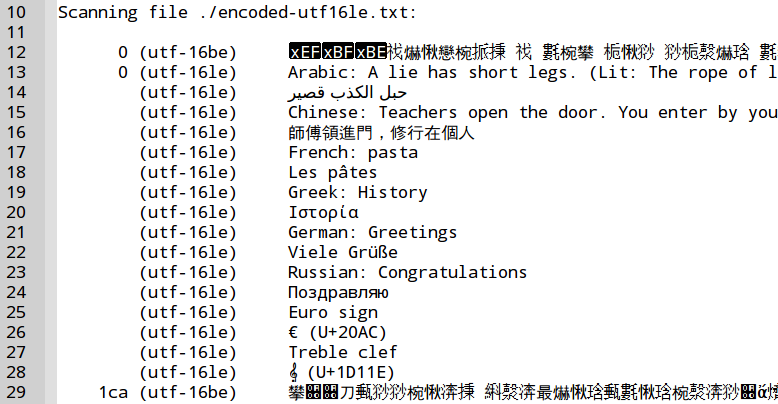
\includegraphics[width=0.80000\textwidth]{images/stringsext-utf-16le-input.png}
\caption{Strings­ext's output with UTF-16le encoded input}
\end{figure}

In the \protect\hyperlink{stringsext-utf-16le-input}{figure\_title} is
interesting to notice, that the UTF-16BE scanner in line 29 restarts at
offset \texttt{0xca}. The above hex-dump of \emph{Strings­ext}'s input
data explains why: the preceding bytes \texttt{df00\ 6500} at position
\texttt{0xc6} are one of the rare invalid code unit combinations in
UTF-16BE (cf.
\protect\hyperlink{utf-16-bit-distribution}{table\_title}). The same
phenomena can be observed in the
\protect\hyperlink{stringsext-utf-16be-input}{figure\_title}.

The \protect\hyperlink{stringsext-utf-16be-input}{figure\_title} and the
\protect\hyperlink{stringsext-utf-16le-input}{figure\_title} show that,
when the right decoder (big-endian or little-endian) is chosen, all
Unicode-characters are recognized and printed correctly. This is huge
improvement compared to \emph{GNU-strings} which failed to recognize any
non-ASCII characters in UTF-16 (cf.
\protect\hyperlink{test-case-strings}{section\_title}).

When the wrong scanner was chosen, we see Chinese and Japanese
characters. These false positives are very common when scanning for
UTF-16 characters. The reason is not the scanner, but an inherent
property of the UTF-16 encoding: Almost every possible byte combination
maps to a valid UTF-16 character! Only some very few byte sequences are
invalid: ``Because surrogate code points are not Unicode scalar values,
isolated UTF-16 code units in the range \texttt{0xD800..0xDFFF} are
ill-formed {[}\protect\hyperlink{unicodeconsortium2016}{18 p.~160}{]}''.
Nevertheless, even code units in this invalid range can appear as
\emph{surrogate pairs} as shown in the last line of the following table:

\begin{longtable}[]{@{}ll@{}}
\caption{UTF-16 Bit distribution}\tabularnewline
\toprule
\begin{minipage}[b]{0.38\columnwidth}\raggedright\strut
Unicode scalar value (code point)\strut
\end{minipage} & \begin{minipage}[b]{0.56\columnwidth}\raggedright\strut
UTF-16-BE code units\strut
\end{minipage}\tabularnewline
\midrule
\endfirsthead
\toprule
\begin{minipage}[b]{0.38\columnwidth}\raggedright\strut
Unicode scalar value (code point)\strut
\end{minipage} & \begin{minipage}[b]{0.56\columnwidth}\raggedright\strut
UTF-16-BE code units\strut
\end{minipage}\tabularnewline
\midrule
\endhead
\begin{minipage}[t]{0.38\columnwidth}\raggedright\strut
\texttt{xxxxxxxx\ xxxxxxxx}\\
(no code points in\\
\texttt{110111000\ 00000000}\\
\ldots{}​ \texttt{110111111\ 11111111})\strut
\end{minipage} & \begin{minipage}[t]{0.56\columnwidth}\raggedright\strut
\texttt{xxxxxxxx\ xxxxxxxx}\\
(all except\\
\texttt{110111000\ 00000000}\\
\ldots{}​ \texttt{110111111\ 11111111})\strut
\end{minipage}\tabularnewline
\begin{minipage}[t]{0.38\columnwidth}\raggedright\strut
\texttt{000uuuuu\ xxxxxxxx\ \ xxxxxxxx}\strut
\end{minipage} & \begin{minipage}[t]{0.56\columnwidth}\raggedright\strut
surrogate pairs:\\
\texttt{110110ww\ wwxxxxxx\ \ 110111xx\ xxxxxxxx}\\
(with \texttt{wwww\ =\ uuuuu\ -\ 1)}\strut
\end{minipage}\tabularnewline
\bottomrule
\end{longtable}

As we can see from the
\protect\hyperlink{utf-16-bit-distribution}{table\_title}, almost every
possible byte sequence, interpreted as UTF-16 code unit, relates to a
Unicode code point. 96\% of the UTF-16 code units map directly to
Unicode plane 0 (Basic Multilingual Plane BMP) code points. This
explains the big number of false positives. But why do we see so many
Chinese and Japanese characters (CJK)? The reason is simple: there are
just so many of them in plane 0! The range \texttt{0x2E80-0x33FF} is
allocated to the ``CJK Miscellaneous Area'', and the range
\texttt{0x3400-0x9FFF} to the ``CJKV Unified Ideographs Area''
{[}\protect\hyperlink{unicodeconsortium2016}{18 p.~85}{]} covering 29055
code units out of 63488 possible code units. This means the probability
of encountering CJKV symboles in a random byte stream, interpreted as
UTF-16, is 44\%. In a stream with ASCII text this probability is even
much higher and can get close to 100\% because alphabetical letters in
ASCII are encoded as \texttt{0x41}-\texttt{0x7a}. When these bytes are
interpreted as high bytes of UTF-16 code units, the result always points
in the CJKV Unicode range.

In the context of forensic examination, false positives are highly
undesirable. A practicable solution could be to restrict the output of
scanners by setting up additional filter criteria: for example the user
could limit his search to a certain Unicode code block. This solution is
out of the scope of this work and considered as future potential
extension.

\begin{quote}
\textbf{Note}

As of \emph{Stringsext} version 1.1 \footnote{This present document
  describes \emph{Stringsext} 1.0. The new Unicode-range-filter feature
  released with \emph{Stringsext} version 1.1 was published after the
  writing of this thesis.}, the \texttt{-\/-encoding} option interprets
specifiers limiting the search scope to a range of Unicode blocks.\\
For example \texttt{-\/-encoding\ utf-16le,8,U+0..U+3ff} searches for
strings encoded in UTF-16 Little Endian being at least 8 bytes long and
containing only Unicode code-points in the range from \texttt{U+0} to
\texttt{U+3ff}. Please consult the man-page for details.
\end{quote}

\subsection{User documentation}\label{_user_documentation}

The following table shows the \emph{man-page} user documentation. It is
typeset as \emph{reStructuredText} and compiled using the \emph{Sphinx}
tool {[}\protect\hyperlink{lehmann2011}{21}{]}.

\begin{longtable}[]{@{}l@{}}
\caption{Manual page - stringsext - version 1.0}\tabularnewline
\toprule
\begin{minipage}[t]{0.97\columnwidth}\raggedright\strut
\textbf{NAME}

stringsext - search for valid strings, decode and print its graphic
characters as UTF-8.

\textbf{stringsext} is a Unicode enhancement of the \emph{GNU strings}
tool with additional functionalities: \textbf{stringsext} recognizes
Cyrillic, CJKV characters and other scripts in all supported
multi-byte-encodings, while \emph{GNU strings} fails in finding any of
these scripts in UTF-16 and many other encodings.

\textbf{SYNOPSIS}

stringsext {[}options{]} {[}-e ENC...{]} {[}-\/-{]} {[}FILE{]}
stringsext {[}options{]} {[}-e ENC...{]} {[}-\/-{]} {[}-{]}

\textbf{DESCRIPTION}

\textbf{stringsext} prints all graphic character sequences in
\emph{FILE} or \emph{stdin} that are at least \emph{MIN} bytes long.

Unlike \emph{GNU strings} \textbf{stringsext} can be configured to
search for valid characters not only in ASCII but also in many other
input encodings, e.g.: utf-8, utf-16be, utf-16le, big5-2003, euc-jp,
koi8-r and many others. \textbf{-\/-list-encodings} shows a list of
valid encoding names based on the WHATWG Encoding Standard. When more
than one encoding is specified, the scan is performed in different
threads simultaneously.

\textbf{stringsext} reads its input data from \textbf{FILE}. With no
\textbf{FILE}, or when \textbf{FILE} is \texttt{-}, it reads standard
input \emph{stdin}.

\textbf{stringsext} is mainly useful for determining the Unicode content
of non-text files.

When invoked with \texttt{stringsext\ -e\ ascii\ -c\ i}
\textbf{stringsext} can be used as \emph{GNU strings} replacement.

\textbf{OPTIONS}

\begin{description}
\item[\textbf{-c} \emph{MODE}, \textbf{-\/-control-chars}=\emph{MODE}]
Determine if and how control characters are printed.

The search algorithm first scans for valid character sequences which are
then are re-encoded into UTF-8 strings containing graphical (printable)
and control (non-printable) characters.

When \emph{MODE} is set to \textbf{p} all valid (control and graphic)
characters are printed. Warning: Control characters may contain a
harmful payload. An attacker may exploit a vulnerability of your
terminal or post processing software. Use with caution.

\emph{MODE} \textbf{r} will never print any control character but
instead indicate their position: Control characters in valid strings are
first grouped and then replaced with the Unicode replacement character
'�' (U+FFFD). This mode is most useful together with \textbf{-\/-radix}
because it keeps the whole valid character sequence in one line allowing
post-processing the output with line oriented tools like \texttt{grep}.
To ease post-processing, the output in MODE \textbf{r} is formatted
slightly different from other modes: instead of indenting the
byte-counter, the encoding name and the found string with \emph{spaces}
as separator, only one \emph{tab} is inserted.

When \emph{MODE} is \textbf{i} all control characters are silently
ignored. They are first grouped and then replaced with a newline
character.

See the output of \textbf{-\/-help} for the default value of
\emph{MODE}.
\item[\textbf{-e} \emph{ENC}, \textbf{-\/-encoding}=\emph{ENC}]
Set (multiple) input search encodings. Encoding names \emph{ENC} are
identified according to the WATHWG standard. \textbf{-\/-list-encodings}
prints a list of implemented encodings.

See the output of \textbf{-\/-help} for the default value of \emph{ENC}.
\item[\textbf{-h, -\/-help}]
Print a synopsis of available options and default values.
\item[\textbf{-l, -\/-list-encodings}]
List available encodings as WHATWG Encoding Standard names and exit.
\item[\textbf{-n} \emph{MIN}, \textbf{-\/-bytes}=\emph{MIN}]
Print only strings at least \emph{min} bytes long. The length is
measured as UTF-8 byte-string. \textbf{-\/-help} shows the default
value.
\item[\textbf{-p} \emph{FILE}, \textbf{-\/-output}=\emph{FILE}]
Print to \emph{FILE} instead of \emph{stdout}.
\item[\textbf{-t} \emph{RADIX}, \textbf{-\/-radix}=\emph{RADIX}]
Print the offset within the file before each valid string. The single
character argument specifies the radix of the offset: \textbf{o} for
octal, \textbf{x} for hexadecimal, or \textbf{d} for decimal. When a
valid string is split into several graphic character sequences the
cut-off point is labelled according to \textbf{-\/-control-chars} but no
additional offset is printed for each graphic character sequence.

The exception to the above is \textbf{-\/-encoding=ascii
-\/-control-chars=i} for which the offset is always printed before each
graphic character sequence.

When the output of \textbf{stringsext} is piped to another filter you
may consider \textbf{-\/-control-chars=r} to keep multi-line strings in
one line.
\item[\textbf{-V, -\/-version}]
Print version info and exit.
\end{description}

\textbf{EXIT STATUS}

\begin{description}
\item[\textbf{0}]
Success.
\item[\textbf{other values}]
Failure.
\end{description}

\textbf{EXAMPLES}

List available encodings:

stringsext -l

Search for UTF-8 strings and strings in UTF-16 Big Endian encoding:

stringsext -e utf-8 -e utf-16be somefile.bin

Or:

cat somefile.bin \{vbar\} stringsext -e utf-8 -e utf-16be -

The following settings are designed to produce bit-identical output with
\emph{GNU strings}:

stringsext -e ascii -c i \# equals `strings` stringsext -e ascii -c i -t
d \# equals `strings -t d` stringsext -e ascii -c i -t x \# equals
`strings -t x` stringsext -e ascii -c i -t o \# equals `strings -t o`

When used with pipes \texttt{-c\ r} is required:

stringsext -e ascii -e iso-8859-7 -c r somefile.bin \{vbar\} grep
"Ιστορία"

\textbf{LIMITATIONS}

It is guaranteed that all valid string sequences are detected and
printed whatever their size is. However due to potential false positives
when interpreting binary data as multi-byte-strings, it may happen that
the first characters of a valid string may not be recognised
immediately. In practice, this effect occurs very rarely and the scanner
synchronises with the correct character boundaries quickly.

When the size of a valid string exceeds FLAG\_BYTES\_MAX bytes it may be
split into two or more strings and then printed separately. Note that
this limitation refers to the \emph{valid} string size and not to the
\emph{graphic} string size which may be shorter. If a valid string is
longer than WIN\_LEN bytes then it is always split. To know the values
of the constants please refer to the definition in the source code of
your \textbf{stringsext} build. Original values are: FLAG\_BYTES\_MAX =
6144 bytes, WIN\_LEN = 14342 bytes.

\textbf{RESOURCES}

\textbf{Project website:} https://github.com/getreu/stringsext

\textbf{COPYING}

Copyright (C) 2016 Jens Getreu

Licensed under the Apache License, Version 2.0 (the "License"); you may
not use this file except in compliance with the License. You may obtain
a copy of the License at

http://www.apache.org/licenses/LICENSE-2.0

Unless required by applicable law or agreed to in writing, software
distributed under the License is distributed on an "AS IS" BASIS,
WITHOUT WARRANTIES OR CONDITIONS OF ANY KIND, either express or implied.
See the License for the specific language governing permissions and
limitations under the License.\strut
\end{minipage}\tabularnewline
\bottomrule
\end{longtable}

\hypertarget{_benchmarking_and_field_experiment}{\subsection{Benchmarking
and field experiment}\label{_benchmarking_and_field_experiment}}

Rust's build in benchmarking feature allows to clock the time of unit
testing code. At the time of this writing this feature is only available
with the ``nightly'' distribution of the Rust compiler. It is especially
valuable when used together with the \emph{test driven development
method} (cf.
\protect\hyperlink{_test_driven_development}{section\_title}): First the
programmer implements the unit testing code for a new feature. The
second step consists in finding alternative solutions to implement this
new feature. Using Rust's benchmarking the programmer can take
performance consideration into account at very early state when he is
still exploring alternative solutions for the to be tested unit.

A second approach to benchmark software is to monitor the system
resource usage of the running binary. The Linux-tool \texttt{time} runs
programs and summarize system resource usage. This way we can compare
the performance of \emph{GNU-strings} and \emph{Stringsext}. For this
purpose the following script runs a series of 6 benchmark tests. In
benchmark test 2 \emph{Stringsext} is launched with only one ASCII
scanner producing the same output as \emph{GNU-strings} in benchmark
test 1.

\begin{quote}
\textbf{Important}

The ``Field experiment 1'' compares the output of \emph{GNU-strings}
with the output of \emph{Strings­ext} in ASCII-only mode on real-life
data. Both are expected to be identical.
\end{quote}

The benchmark tests 3 to 5 are designed to study how \emph{Strings­ext}
scale with more than one ASCII-scanner. The last benchmark 6 is a more
realistic test case with 4 different scanners: ASCII, UTF-8, UTF-16BE
and UTF-16LE.

All test operate on the same input data: a partition image with a Linux
kernel \texttt{dev-sda.raw}.

\textbf{Benchmark script.}

\begin{Shaded}
\begin{Highlighting}[]
\CommentTok{#!/bin/sh}
\VariableTok{FILE=}\NormalTok{dev-sda.raw}
\VariableTok{BMARK=}\StringTok{"}\VariableTok{$1}\StringTok{-benchmark.txt"}

\BuiltInTok{echo} \StringTok{"}\VariableTok{$(}\ExtensionTok{./stringsext} \NormalTok{-V}\VariableTok{)}\StringTok{"} \OperatorTok{>>}\StringTok{"}\VariableTok{$BMARK}\StringTok{"}
\BuiltInTok{echo} \StringTok{"Inputfile: }\VariableTok{$(}\FunctionTok{ls} \NormalTok{-l }\VariableTok{$FILE)}\StringTok{"} \OperatorTok{>>}\StringTok{"}\VariableTok{$BMARK}\StringTok{"}

\BuiltInTok{echo} \StringTok{"\textbackslash{}n\textbackslash{}nBenchmark 1"} \OperatorTok{>>}\StringTok{"}\VariableTok{$BMARK}\StringTok{"}
\BuiltInTok{time} \NormalTok{-vao }\StringTok{"}\VariableTok{$BMARK}\StringTok{"} \NormalTok{strings -n 10 -t x }\VariableTok{$FILE} \NormalTok{\textbackslash{}}
    \OperatorTok{>} \StringTok{"}\VariableTok{$1}\StringTok{-input_}\VariableTok{$FILE}\StringTok{-output_orig.txt"}

\BuiltInTok{echo} \StringTok{"\textbackslash{}n\textbackslash{}nBenchmark 2"} \OperatorTok{>>}\StringTok{"}\VariableTok{$BMARK}\StringTok{"}
\BuiltInTok{time} \NormalTok{-vao }\StringTok{"}\VariableTok{$BMARK}\StringTok{"} \NormalTok{./stringsext -c i -n 10 -e ascii -t x }\VariableTok{$FILE} \NormalTok{\textbackslash{}}
    \OperatorTok{>} \StringTok{"}\VariableTok{$1}\StringTok{-input_}\VariableTok{$FILE}\StringTok{-output_1scanner.txt"}

\BuiltInTok{echo} \StringTok{"\textbackslash{}n\textbackslash{}nField experiment 1"} \OperatorTok{>>}\StringTok{"}\VariableTok{$BMARK}\StringTok{"}
\FunctionTok{cmp} \NormalTok{--silent }\StringTok{"}\VariableTok{$1}\StringTok{-input_}\VariableTok{$FILE}\StringTok{-output_orig.txt"} \NormalTok{\textbackslash{}}
             \StringTok{"}\VariableTok{$1}\StringTok{-input_}\VariableTok{$FILE}\StringTok{-output_1scanner.txt"}
\KeywordTok{if}\BuiltInTok{ [} \VariableTok{$?} \OtherTok{-eq} \NormalTok{0}\BuiltInTok{ ]} \NormalTok{; }\KeywordTok{then}
   \BuiltInTok{echo} \StringTok{"    Success: Output of benchmark 1 and 2 is identical."} \NormalTok{\textbackslash{}}
        \OperatorTok{>>} \StringTok{"}\VariableTok{$BMARK}\StringTok{"}
\KeywordTok{else}
   \BuiltInTok{echo} \StringTok{"    FAILED! strings' and stringsext's output is different!"} \NormalTok{\textbackslash{}}
        \KeywordTok{|}\FunctionTok{tee} \NormalTok{-a }\StringTok{"}\VariableTok{$BMARK}\StringTok{"}  \KeywordTok{&&}  \BuiltInTok{exit} \NormalTok{1}
\KeywordTok{fi}

\BuiltInTok{echo} \StringTok{"\textbackslash{}n\textbackslash{}nBenchmark 3"} \OperatorTok{>>}\StringTok{"}\VariableTok{$BMARK}\StringTok{"}
\BuiltInTok{time} \NormalTok{-vao }\StringTok{"}\VariableTok{$BMARK}\StringTok{"}  \NormalTok{./stringsext -n 10 -e ascii -e ascii -t x }\VariableTok{$FILE} \NormalTok{\textbackslash{}}
    \OperatorTok{>} \StringTok{"}\VariableTok{$1}\StringTok{-input_}\VariableTok{$FILE}\StringTok{-output_2ascii.txt"}

\BuiltInTok{echo} \StringTok{"\textbackslash{}n\textbackslash{}nBenchmark 4"} \OperatorTok{>>}\StringTok{"}\VariableTok{$BMARK}\StringTok{"}
\BuiltInTok{time} \NormalTok{-vao }\StringTok{"}\VariableTok{$BMARK}\StringTok{"}  \NormalTok{./stringsext -n 10 -e ascii -e ascii -e ascii -t x \textbackslash{}}
    \VariableTok{$FILE}  \OperatorTok{>} \StringTok{"}\VariableTok{$1}\StringTok{-input_}\VariableTok{$FILE}\StringTok{-output_3ascii.txt"}

\BuiltInTok{echo} \StringTok{"\textbackslash{}n\textbackslash{}nBenchmark 5"} \OperatorTok{>>}\StringTok{"}\VariableTok{$BMARK}\StringTok{"}
\BuiltInTok{time} \NormalTok{-vao }\StringTok{"}\VariableTok{$BMARK}\StringTok{"}  \NormalTok{./stringsext -n 10 -e ascii -e ascii -e ascii \textbackslash{}}
    \NormalTok{-e ascii -t x }\VariableTok{$FILE} \OperatorTok{>} \StringTok{"}\VariableTok{$1}\StringTok{-input_}\VariableTok{$FILE}\StringTok{-output_4ascii.txt"}

\BuiltInTok{echo} \StringTok{"\textbackslash{}n\textbackslash{}nBenchmark 6"} \OperatorTok{>>}\StringTok{"}\VariableTok{$BMARK}\StringTok{"}
\BuiltInTok{time} \NormalTok{-vao }\StringTok{"}\VariableTok{$BMARK}\StringTok{"}  \NormalTok{./stringsext -n 10 -e ascii -e utf-8 -e utf-16be \textbackslash{}}
    \NormalTok{-e utf-16le -t x }\VariableTok{$FILE} \OperatorTok{>} \StringTok{"}\VariableTok{$1}\StringTok{-input_}\VariableTok{$FILE}\StringTok{-output_4scanners.txt"}

\BuiltInTok{echo} \StringTok{"\textbackslash{}n\textbackslash{}n\textbackslash{}n"} \OperatorTok{>>}\StringTok{"}\VariableTok{$BMARK}\StringTok{"}
\end{Highlighting}
\end{Shaded}

The script is executed on a laptop with an Intel Core i5-2540M, 2.60GHz
CPU.

\textbf{Benchmark results.}

\begin{Shaded}
\begin{Highlighting}[]
\ExtensionTok{Version} \NormalTok{0.9.4, (c) }\ExtensionTok{Jens} \NormalTok{Getreu, 2016}
\ExtensionTok{Inputfile}\NormalTok{:-rw-rw---- 1 jens myworkers 536870912 Aug 18 09:12 dev-sda.raw}

\ExtensionTok{Benchmark} \NormalTok{1}
    \ExtensionTok{Command} \NormalTok{being timed: }\StringTok{"strings -n 10 -t x dev-sda.raw"}
    \ExtensionTok{User} \NormalTok{time (seconds)}\BuiltInTok{:} \NormalTok{4.65}
    \ExtensionTok{System} \NormalTok{time (seconds)}\BuiltInTok{:} \NormalTok{0.06}
    \ExtensionTok{Percent} \NormalTok{of CPU this job got: 99%}
    \ExtensionTok{Elapsed} \NormalTok{(wall clock) }\BuiltInTok{time} \NormalTok{(h:mm:ss or m:ss)}\BuiltInTok{:} \NormalTok{0:04.72}
    \ExtensionTok{Maximum} \NormalTok{resident set size (kbytes)}\BuiltInTok{:} \NormalTok{2616}
    \ExtensionTok{File} \NormalTok{system outputs: 8552}

\ExtensionTok{Benchmark} \NormalTok{2}
    \ExtensionTok{Command} \NormalTok{being timed: }\StringTok{"./stringsext -c i -n 10 -e ascii -t x dev-sda.raw"}
    \ExtensionTok{User} \NormalTok{time (seconds)}\BuiltInTok{:} \NormalTok{11.26}
    \ExtensionTok{System} \NormalTok{time (seconds)}\BuiltInTok{:} \NormalTok{1.01}
    \ExtensionTok{Percent} \NormalTok{of CPU this job got: 106%}
    \ExtensionTok{Elapsed} \NormalTok{(wall clock) }\BuiltInTok{time} \NormalTok{(h:mm:ss or m:ss)}\BuiltInTok{:} \NormalTok{0:11.49}
    \ExtensionTok{Maximum} \NormalTok{resident set size (kbytes)}\BuiltInTok{:} \NormalTok{13032}
    \ExtensionTok{File} \NormalTok{system outputs: 8552}

\ExtensionTok{Field} \NormalTok{experiment 1}
    \ExtensionTok{Success}\NormalTok{: Output of benchmark 1 and 2 is identical.}

\ExtensionTok{Benchmark} \NormalTok{3}
    \ExtensionTok{Command} \NormalTok{being timed: }\StringTok{"./stringsext -n 10 -e ascii -e ascii -t x dev-sda.raw"}
    \ExtensionTok{User} \NormalTok{time (seconds)}\BuiltInTok{:} \NormalTok{31.56}
    \ExtensionTok{System} \NormalTok{time (seconds)}\BuiltInTok{:} \NormalTok{1.52}
    \ExtensionTok{Percent} \NormalTok{of CPU this job got: 195%}
    \ExtensionTok{Elapsed} \NormalTok{(wall clock) }\BuiltInTok{time} \NormalTok{(h:mm:ss or m:ss)}\BuiltInTok{:} \NormalTok{0:16.91}
    \ExtensionTok{Maximum} \NormalTok{resident set size (kbytes)}\BuiltInTok{:} \NormalTok{19604}
    \ExtensionTok{File} \NormalTok{system outputs: 23176}

\ExtensionTok{Benchmark} \NormalTok{4}
    \ExtensionTok{Command} \NormalTok{being timed: }\StringTok{"./stringsext -n 10 -e ascii -e ascii -e ascii -t x dev-sda.raw"}
    \ExtensionTok{User} \NormalTok{time (seconds)}\BuiltInTok{:} \NormalTok{49.86}
    \ExtensionTok{System} \NormalTok{time (seconds)}\BuiltInTok{:} \NormalTok{2.51}
    \ExtensionTok{Percent} \NormalTok{of CPU this job got: 248%}
    \ExtensionTok{Elapsed} \NormalTok{(wall clock) }\BuiltInTok{time} \NormalTok{(h:mm:ss or m:ss)}\BuiltInTok{:} \NormalTok{0:21.08}
    \ExtensionTok{Maximum} \NormalTok{resident set size (kbytes)}\BuiltInTok{:} \NormalTok{26388}
    \ExtensionTok{File} \NormalTok{system outputs: 34752}

\ExtensionTok{Benchmark} \NormalTok{5}
    \ExtensionTok{Command} \NormalTok{being timed: }\StringTok{"./stringsext -n 10 -e ascii -e ascii -e ascii -e ascii -t x dev-sda.raw"}
    \ExtensionTok{User} \NormalTok{time (seconds)}\BuiltInTok{:} \NormalTok{71.66}
    \ExtensionTok{System} \NormalTok{time (seconds)}\BuiltInTok{:} \NormalTok{3.09}
    \ExtensionTok{Percent} \NormalTok{of CPU this job got: 312%}
    \ExtensionTok{Elapsed} \NormalTok{(wall clock) }\BuiltInTok{time} \NormalTok{(h:mm:ss or m:ss)}\BuiltInTok{:} \NormalTok{0:23.89}
    \ExtensionTok{Maximum} \NormalTok{resident set size (kbytes)}\BuiltInTok{:} \NormalTok{32692}
    \ExtensionTok{File} \NormalTok{system outputs: 46336}

\ExtensionTok{Benchmark} \NormalTok{6}
    \ExtensionTok{Command} \NormalTok{being timed: }\StringTok{"./stringsext -n 10 -e ascii -e utf-8 -e utf-16be -e utf-16le -t x dev-sda.raw"}
    \ExtensionTok{User} \NormalTok{time (seconds)}\BuiltInTok{:} \NormalTok{53.00}
    \ExtensionTok{System} \NormalTok{time (seconds)}\BuiltInTok{:} \NormalTok{9.29}
    \ExtensionTok{Percent} \NormalTok{of CPU this job got: 225%}
    \ExtensionTok{Elapsed} \NormalTok{(wall clock) }\BuiltInTok{time} \NormalTok{(h:mm:ss or m:ss)}\BuiltInTok{:} \NormalTok{0:27.64}
    \ExtensionTok{Maximum} \NormalTok{resident set size (kbytes)}\BuiltInTok{:} \NormalTok{18896}
    \ExtensionTok{File} \NormalTok{system outputs: 1177360}
\end{Highlighting}
\end{Shaded}

\begin{longtable}[]{@{}llllll@{}}
\caption{Benchmark result synopsis}\tabularnewline
\toprule
\begin{minipage}[b]{0.14\columnwidth}\raggedright\strut
Benchmark\strut
\end{minipage} & \begin{minipage}[b]{0.14\columnwidth}\raggedright\strut
\% of CPU\strut
\end{minipage} & \begin{minipage}[b]{0.14\columnwidth}\raggedright\strut
Clock\strut
\end{minipage} & \begin{minipage}[b]{0.14\columnwidth}\raggedright\strut
Threads\strut
\end{minipage} & \begin{minipage}[b]{0.14\columnwidth}\raggedright\strut
\% CPU ideal\strut
\end{minipage} & \begin{minipage}[b]{0.14\columnwidth}\raggedright\strut
Clock adjusted\strut
\end{minipage}\tabularnewline
\midrule
\endfirsthead
\toprule
\begin{minipage}[b]{0.14\columnwidth}\raggedright\strut
Benchmark\strut
\end{minipage} & \begin{minipage}[b]{0.14\columnwidth}\raggedright\strut
\% of CPU\strut
\end{minipage} & \begin{minipage}[b]{0.14\columnwidth}\raggedright\strut
Clock\strut
\end{minipage} & \begin{minipage}[b]{0.14\columnwidth}\raggedright\strut
Threads\strut
\end{minipage} & \begin{minipage}[b]{0.14\columnwidth}\raggedright\strut
\% CPU ideal\strut
\end{minipage} & \begin{minipage}[b]{0.14\columnwidth}\raggedright\strut
Clock adjusted\strut
\end{minipage}\tabularnewline
\midrule
\endhead
\begin{minipage}[t]{0.14\columnwidth}\raggedright\strut
no.\strut
\end{minipage} & \begin{minipage}[t]{0.14\columnwidth}\raggedright\strut
this job got\strut
\end{minipage} & \begin{minipage}[t]{0.14\columnwidth}\raggedright\strut
measured elapsed time\strut
\end{minipage} & \begin{minipage}[t]{0.14\columnwidth}\raggedright\strut
scanner + merger/printer\strut
\end{minipage} & \begin{minipage}[t]{0.14\columnwidth}\raggedright\strut
required for optimal speed\strut
\end{minipage} & \begin{minipage}[t]{0.14\columnwidth}\raggedright\strut
adjusted for throttling\strut
\end{minipage}\tabularnewline
\begin{minipage}[t]{0.14\columnwidth}\raggedright\strut
1\strut
\end{minipage} & \begin{minipage}[t]{0.14\columnwidth}\raggedright\strut
99\%\strut
\end{minipage} & \begin{minipage}[t]{0.14\columnwidth}\raggedright\strut
\emph{00:04.72}\strut
\end{minipage} & \begin{minipage}[t]{0.14\columnwidth}\raggedright\strut
1\strut
\end{minipage} & \begin{minipage}[t]{0.14\columnwidth}\raggedright\strut
100\%\strut
\end{minipage} & \begin{minipage}[t]{0.14\columnwidth}\raggedright\strut
00:04.67\strut
\end{minipage}\tabularnewline
\begin{minipage}[t]{0.14\columnwidth}\raggedright\strut
2\strut
\end{minipage} & \begin{minipage}[t]{0.14\columnwidth}\raggedright\strut
106\%\strut
\end{minipage} & \begin{minipage}[t]{0.14\columnwidth}\raggedright\strut
\emph{00:11.49}\strut
\end{minipage} & \begin{minipage}[t]{0.14\columnwidth}\raggedright\strut
1+1\strut
\end{minipage} & \begin{minipage}[t]{0.14\columnwidth}\raggedright\strut
106\%\strut
\end{minipage} & \begin{minipage}[t]{0.14\columnwidth}\raggedright\strut
\textbf{00:11.49}\strut
\end{minipage}\tabularnewline
\begin{minipage}[t]{0.14\columnwidth}\raggedright\strut
3\strut
\end{minipage} & \begin{minipage}[t]{0.14\columnwidth}\raggedright\strut
195\%\strut
\end{minipage} & \begin{minipage}[t]{0.14\columnwidth}\raggedright\strut
00:16.91\strut
\end{minipage} & \begin{minipage}[t]{0.14\columnwidth}\raggedright\strut
2+1\strut
\end{minipage} & \begin{minipage}[t]{0.14\columnwidth}\raggedright\strut
212\%\strut
\end{minipage} & \begin{minipage}[t]{0.14\columnwidth}\raggedright\strut
\textbf{00:15.55}\strut
\end{minipage}\tabularnewline
\begin{minipage}[t]{0.14\columnwidth}\raggedright\strut
4\strut
\end{minipage} & \begin{minipage}[t]{0.14\columnwidth}\raggedright\strut
248\%\strut
\end{minipage} & \begin{minipage}[t]{0.14\columnwidth}\raggedright\strut
00:21.08\strut
\end{minipage} & \begin{minipage}[t]{0.14\columnwidth}\raggedright\strut
3+1\strut
\end{minipage} & \begin{minipage}[t]{0.14\columnwidth}\raggedright\strut
336\%\strut
\end{minipage} & \begin{minipage}[t]{0.14\columnwidth}\raggedright\strut
\textbf{00:15.56}\strut
\end{minipage}\tabularnewline
\begin{minipage}[t]{0.14\columnwidth}\raggedright\strut
5\strut
\end{minipage} & \begin{minipage}[t]{0.14\columnwidth}\raggedright\strut
312\%\strut
\end{minipage} & \begin{minipage}[t]{0.14\columnwidth}\raggedright\strut
00:23.89\strut
\end{minipage} & \begin{minipage}[t]{0.14\columnwidth}\raggedright\strut
4+1\strut
\end{minipage} & \begin{minipage}[t]{0.14\columnwidth}\raggedright\strut
448\%\strut
\end{minipage} & \begin{minipage}[t]{0.14\columnwidth}\raggedright\strut
\textbf{00:16.64}\strut
\end{minipage}\tabularnewline
\begin{minipage}[t]{0.14\columnwidth}\raggedright\strut
6\strut
\end{minipage} & \begin{minipage}[t]{0.14\columnwidth}\raggedright\strut
225\%\strut
\end{minipage} & \begin{minipage}[t]{0.14\columnwidth}\raggedright\strut
00:27.64\strut
\end{minipage} & \begin{minipage}[t]{0.14\columnwidth}\raggedright\strut
4+1\strut
\end{minipage} & \begin{minipage}[t]{0.14\columnwidth}\raggedright\strut
448\%\strut
\end{minipage} & \begin{minipage}[t]{0.14\columnwidth}\raggedright\strut
\textbf{00:13.88}\strut
\end{minipage}\tabularnewline
\bottomrule
\end{longtable}

\begin{enumerate}
\def\labelenumi{\arabic{enumi}.}
\item
  When scanning only ASCII, \emph{GNU-strings} is 2.4 times faster than
  \emph{Stringsext}. (Compare ``\% of CPU'' benchmark 1 and 2).
\item
  The \emph{merger/printer} thread consumes approximately 6\% of the
  processor resources of one ASCII scanner thread.
\item
  In benchmark 4-6 \emph{Stringsext} is slowed down because of missing
  hardware resources. (Compare column ``\% of CPU` this job got'' and
  ``\% CPU ideal, required for optimal speed''). The threads are also
  throttled down because the processor temperature exceeds 80°C.
\item
  The column ``Clock adjusted'' show the adjusted value for throttling
  slow down we expect for a system with better hardware resources. The
  benchmarks where run on a laptop with an Intel Core i5-2540M CPU at
  2.60GHz. Although this processor can run four threads concurrently,
  all threads have to share only two cores.
\item
  In line with expectations, the ``maximum resident set size'' of
  \emph{Strings­ext} depends on the number of threads launched. Its
  highest value of 32,7MB was observed in benchmark 5.
\item
  The ``Field experiment 1'' succeeds: \emph{GNU-strings}' output and
  \emph{Stringsext}'s output in ASCII-only mode are identical.
\end{enumerate}

\textbf{Conclusion.}

When launched as pure ASCII scanner \emph{Stringsext} produces the same
output as \emph{GNU-strings}, but 2.4 times slower. This result is very
satisfactory: \emph{Strings­ext}'s ASCII-only mode is only one special
usage scenario among many others requiring complex time costly
computing. When scanning for other encodings or for more than one
encoding in parallel \emph{Strings­ext} can play off its particular
strengths. It is best run on modern hardware with four or more kernels.

\subsection{Product evaluation}\label{_product_evaluation}

In the
\protect\hyperlink{_benchmarking_and_field_experiment}{section\_title}
we could convince ourselves that \emph{Strings­ext} produces accurate
results timely. But how do matters stand with the other requirements
defined in the \protect\hyperlink{_specifications}{???}? Specifically:

\begin{description}
\item[{\protect\hyperlink{user-interface}{section\_title}}]
\emph{The user interface of Strings­ext should reproduce GNU-strings'
user interface as close as possible.}\\
The command-line-options: \texttt{-\/-bytes}, \texttt{-\/-radix},
\texttt{-\/-help}, \texttt{-\/-version}, \texttt{-n}, \texttt{-t} and
\texttt{-V} have the same meaning and syntax. The syntax of
\texttt{-\/-encoding} takes into account \emph{Stringsext's} advanced
encoding support. The option \texttt{-w} is replaced by
\texttt{-c\ MODE} offering a better output control.
\item[{\protect\hyperlink{character-encoding-support}{section\_title}}]
\emph{Besides ASCII, Strings­ext should support common multi-byte
encodings like UTF-8, UTF-16 big endian, UTF-16 little endian, KOI8-R,
KOI8U, BIG5, EUC-JP and others.}\\
All the listed encodings are covered (see details in the
\protect\hyperlink{decoder}{section\_title}). The found strings in
multiple encodings are merged and presented in chronological order. The
user can specify more than one encoding at the same time.
\item[{\protect\hyperlink{req-concurrent}{section\_title}}]
\emph{Each search encoding specified by the user is assigned to a
separate thread.}\\
This design specification is meet and detailed in the
\protect\hyperlink{_concurrency}{section\_title}.
\item[{\protect\hyperlink{req-batch-processing}{section\_title}}]
\emph{All scanners operate simultaneously on the same chunk of the
search field.}\\
To meet this requirement a proprietary input reader with a circular
buffer is implemented (cf.
\protect\hyperlink{_polymorphic_io}{section\_title}).
\item[{\protect\hyperlink{req-merge-findings}{section\_title}}]
\emph{When all threads' findings are collected, the merging algorithm
brings them in chronological order.}\\
Different alternatives had been explored (cf.
\protect\hyperlink{_merging_vectors}{section\_title}). The implemented
solution uses the \texttt{kmerge()}-function of the
\emph{rust/itertools} library.
\item[{\protect\hyperlink{req-post-treatment}{section\_title}}]
\emph{Strings­ext should have at least one print mode allowing
post-treatment with line-oriented tools like \texttt{grep} or
\texttt{agrep}.}\\
The command-line-options \texttt{-\/-radix=x}
\texttt{-\/-control-chars=r} print the offset of the finding, a tab
character, the encoding name, a tab character and the found string in
one line. Control characters in the found string are replaced with '�'
(U+FFFD). This output format facilitates post-treatment with
line-orientated tools and spreadsheet applications.
\item[{\protect\hyperlink{automated-test-framework}{section\_title}}]
\emph{Automated unit tests guaranty correct results for the implemented
test cases. Furthermore, the chosen methodology makes sure that the
tests are working as intended.}\\
\emph{Stringsext} has 17 unit tests. The chosen \emph{test driven
development} method (cf.
\protect\hyperlink{_development_cycle}{section\_title}) guarantees that
the unit tests work as intended.
\item[{\protect\hyperlink{functionality-oriented-validation}{section\_title}}]
\emph{The same hard-disk image of approximate 500MB is analysed twice:
first with GNU-strings then with Strings­ext. If both outputs are
identical, the test is passed.}\\
This test, hereinafter referred to as ``Field experiment 1'' is executed
with success and discussed in the
\protect\hyperlink{_benchmarking_and_field_experiment}{section\_title}.
\item[{\protect\hyperlink{efficiency-and-speed}{section\_title}}]
To address this requirement \emph{Strings­ext} is developed in the
system programming language Rust (cf. \protect\hyperlink{rust}{???}).
The satisfactory results are described and discussed in the
\protect\hyperlink{_benchmarking_and_field_experiment}{section\_title}.
\item[{\protect\hyperlink{security2}{section\_title}}]
This matter is addressed e.g. by choosing the new system programming
language \emph{Rust} offering various compile-time security guarantees
(cf. \protect\hyperlink{rust}{???}). See also the analysis and the
discussion in the \protect\hyperlink{security1}{section\_title} and the
\protect\hyperlink{security2}{section\_title}.
\end{description}

\textbf{Conclusion.}

\emph{Strings­ext} meets all requirements defined in the
\protect\hyperlink{_specifications}{???}. Because of the inherent
properties of the UTF-16 encoding, the UTF-16 scanners produce many
false positives when run over binary data. A possible solution is
suggested at the end of the
\protect\hyperlink{_utf_16_encoded_input}{section\_title}.

\subsection{User feedback}\label{_user_feedback}

Before publishing \emph{Strings­ext}, a beta-version had been tested by
a small group of forensic practitioners. In addition, the participants
were invited to report back about desirable extensions or missing
features:

\begin{quote}
\begin{enumerate}
\def\labelenumi{\arabic{enumi}.}
\item
  String decoding based \url{https://tools.ietf.org/html/rfc4648}
  (Base64 and others)~
\item
  Base58~decoding~
\item
  It would be nice that the list option \texttt{-l} displayed the
  supported encodings in alphabetic order, this would make easier to
  find the option we are looking for.
\end{enumerate}

---  User feedback: feature requests
\end{quote}

Regarding additional encodings: \emph{Strings­ext} is designed to be
extensible. Adding further encodings other than the ones listed in the
\protect\hyperlink{decoder}{section\_title} is beyond the scope of this
project, but it is made easy: As working sample encoding extension
\texttt{ASCII\_GRAPHIC} can be found in the source code of
\emph{Strings­ext} in \texttt{src/codec/ascii.rs}. The request ``ordered
list'' was implemented in version 0.9.5.

So far \emph{Strings­ext's} search algorithm is based solely on finding
\emph{valid} byte sequences for a given encoding. \emph{Strings­ext} is
a pure \emph{data processing system} in the sense that there are no
semantics weather the resulting graphical character sequences make any
``sense''. The following suggestion received by email
{[}\protect\hyperlink{frade2016}{22}{]} goes far beyond this limitation.

\begin{quote}
For future development: it would be nice to have some form of automatic
detection of what encodings are more likely to be present in a given
file, or even go further and do automatic detection of language like in
Google translator (maybe you could upload selected words)
{[}\protect\hyperlink{frade2016}{22}{]}.

---  Professor Miguel Frade Computer Science and Communication Research
Centre - Polytechnic Institute of Leiria
\end{quote}

This above idea opens the very interesting research field of
\emph{Computational Linguistics}. Language detection in character
sequences requires a linguistic model of ``what is a word'' in a given
human language. Thus, with the suggested enhancement \emph{Strings­ext}
would become a \emph{language processing system}.

Jurafsky {[}\protect\hyperlink{jurafsky2014}{23 p.~3}{]} illustrates the
conceptual difference between a \emph{data processing system} and a
\emph{language processing system} as follows: ``What distinguishes
language processing applications from other data processing systems is
their use of knowledge of language. Consider the Unix \texttt{wc}
program, which counts the total number of bytes, words, and lines in a
text fi le. When used to count bytes and lines, \texttt{wc} is an
ordinary data processing application. However, when it is used to count
the words in a file, it requires knowledge about what it means to be a
word and thus becomes a language processing system.'' Applied to
\emph{Strings­ext} ``the knowledge about what it means to be a word''
comprises a probabilistic model about the likelihood that a certain
character sequence represent a word in a given human language. It is
clear that the approach is beyond the scope of this project.
Nevertheless, the exiting challenge could be tackled in future research
projects.

\subsection{Licence and distribution}\label{_licence_and_distribution}

\emph{Strings­ext} is licensed under the Apache Licence, Version 2.0;
you may not use this program except in compliance with the Licence. You
may obtain a copy of the Licence at
\texttt{http://www.apache.org/licenses/LICENSE-2.0}. The copyright
remains with the author Jens Getreu.

Unless required by applicable law or agreed to in writing, software
dis­tri­bu­ted under the Licence is distributed on an "AS IS" BASIS,
WITHOUT WARRANTIES OR CONDITIONS OF ANY KIND, either express or implied.
See the Licence for the specific language governing permissions and
limitations under the Licence.

The source code including its inline source documentation is hosted on
Github {[}\protect\hyperlink{getreu2016}{1}{]}:
\texttt{https://github.com/getreu/stringsext}. The project's main page
has links to the developer documentation and to the compiled binaries
for various architectures.

\section{Development process evaluation and
conclusion}\label{_development_process_evaluation_and_conclusion}

Besides the contribution of the new tool \emph{Strings­ext} to the
forensic community a more general consideration is of scientific
interest: Seeing that Rust is a very young programming language: how
well is the Rust ecosystem suited for forensic tool development?

Forensic tools have to fulfil stringent requirements concerning their
quality: In general, huge amount of data has to be processed which leads
to most demanding requirements in terms code efficiency (cf.
\protect\hyperlink{_code_efficiency}{section\_title}). Furthermore, the
data to be analysed is potentially dangerous: it may contain malicious
payload targeting common vulnerabilities (cf.
\protect\hyperlink{security1}{section\_title}). Finally, in order to
fulfil legal requirements forensic tools must be extensively tested.

The present case study confirm my initial hypothesis that Rust addresses
theses requirements (cf. \protect\hyperlink{rust}{???}): Rust, as system
programming language, is designed for code efficiency. Rust's security
guaranties comprise memory safety, the cause for a common category of
vulnerabilities. It's build in unit testing feature supports
\emph{software verification} as defined in the
\protect\hyperlink{_tool_validation}{section\_title}.

Guaranteed memory safety is a core property of Rust's borrow checker:
When a Rust source code compiles, the resulting binary \emph{is}
guaranteed to be memory safe. In consequence, such a binary is immune to
memory safety related attacks: e.g. out-of-bounds read, buffer
over-read, heap-based buffer overflow, improper validation of array
index, improper release of memory before removing last, double free, use
after free. As \emph{Strings­ext} and all its used libraries are solely
Rust components, \emph{Strings­ext} is memory safe.

In the
\protect\hyperlink{_benchmarking_and_field_experiment}{section\_title}
we compared the code efficiency of \emph{GNU-strings} implemented in C
and \emph{Strings­ext} implemented in Rust. When \emph{Strings­ext} is
run in ASCII-only mode, both produce the same output. The field
experiment yielded the expected result, 2.4 times slower but still on
the same scale. However, \emph{Stringsext's} design implies much more
complex computations, hence the result is not surprising.

How about the efficiency of Rust's abstractions and its overall
performance? A good estimation is to compare benchmarks of small and
simple programs. Too complex programs should be avoided for this purpose
because variations of the programmer's skills may bias the result.
According to the ``Computer Language Benchmark Game''
{[}\protect\hyperlink{fulgham2016}{24}{]} Rust and \emph{C/C++} have
similar benchmark results.

Forensic tools have to operate on many architectures. Here enters Rust's
cross-compiling feature on scene:

\begin{quote}
As \emph{Rust} uses the LLVM framework as backend, it is available for
most platforms. \texttt{rust-lang-nursery/rustup.rs}
{[}\protect\hyperlink{anderson2016}{25}{]} is a Rust toolchain
multiplexer. It installs and manages several toolchains in parallel and
presents them all through a single set of tools installed. Thanks to the
LLVM backend, it's always been possible in principle to cross-compile
Rust code: just tell the backend to use a different target! And indeed,
intrepid hackers have put Rust on embedded systems like the Raspberry Pi
3, bare metal ARM, MIPS routers running OpenWRT, and many others.
\end{quote}

As described above, Rust's memory safety guarantee is a huge improvement
in terms of security because a whole category of potential
vulnerabilities can be ruled out from the outset. But memory safety does
not mean bug freeness! Beside the security aspects discussed above, the
correctness of forensic software is crucial (cf.
\protect\hyperlink{_tool_validation}{section\_title}). It is clear that
the overall correctness of a program depend also on the correctness of
every library used. Hence, the question arises whether the Rust
ecosystem is mature enough to meet the ambitious requirements of
forensic software. Indeed, compared to C, Rust's libraries are
relatively young. Here again extensive unit testing revealed to be a
helpful diagnostic method: version 0.4.16 of the brand new
\texttt{kmerge} function, part of the \texttt{itertools} library used in
\emph{Strings­ext}, reversed under rare conditions the first and second
finding. This bug was actually fixed with pull request \#135 (2. Aug.
2016) some days after its appearance. Although the bug-fix was already
committed in Github, the package manager did not know about it, because
no new version of \texttt{itertools} was released yet. On the whole, a
little change in the package reference list \texttt{Cargo.toml} solved
the problem immediately. Finally, it took another week for the corrected
\texttt{itertools} version to be released. So far this was the only time
I encountered a bug in any of the used libraries. One conclusion we can
draw from this experience, is that young libraries are more likely to
have bugs than established ones. It cannot be emphasised enough that,
diligent unit tests help to find most bugs at early state. Also those
present in external libraries. However, unit testing do not help against
memory safety related vulnerabilities, which are typical for C and C++
programs and which can persist in software for decades. It is incumbent
on readers to form their own opinion, I largely prefer accepting the
greater likelihood of manageable bugs related to young Rust libraries,
than the uncertainty of hidden memory safety related vulnerabilities
typical for \emph{C} and \emph{C++}.

Rust code has the reputation that it is easy to read and understand, but
it is hard to write. I subscribe to this point of view. Rust's biggest
strength is that unsafe code does not compile, can be also very
frustrating. Especially when you do not understand the compiler's error
messages. At some stage it even happened, that I run out of ideas how to
fix a particular problem. Fortunately, the Rust Internet community is
very supporting and helpful. In the meantime, also Rust's error messages
improved with version 1.12 and Rust's documentation is steadily updated
and enhanced.

The benefits of \emph{unit testing} had been stressed throughout this
work. The chosen software development method for this project was the
\emph{test driven development} method where \emph{unit testing} is the
key element. Contrary to other methods unit tests and the to be tested
code is always programmed by the same person. The
\protect\hyperlink{_test_driven_development}{section\_title} describes
the method more in detail and shows why it was good choice under the
given circumstances. However, other methods may be as suitable depending
on the organisational structure of the programmer team.

\textbf{Conclusion.}

Looking back, Rust was a very good choice for the present project, even
though batch processing of multi-bytes character streams revealed to be
far more complex than expected. Additionally, concurrent programming in
Rust posed a formidable hurdle at the beginning. Fortunately, it did
prove to be helpful to contact the Rust community for their friendly
assistance. In addition, for a not so experienced Rust programmer it is
reassuring to know that when a complex piece of code finally compiles,
it is memory safe. The same reasoning applies when a programmer has to
refactor existing code. I often had a queasy feeling when I had to work
on other people C code. Do I free the memory at the right moment? Is
this pointer still valid? Rust's ownership paradigm resolves this
uncertainty. When it compiles, then it is memory safe. Furthermore, Rust
is especially suitable for bigger projects where several programmers
contribute to the same code. And this is particularly true when
developing forensic software with its high quality standards.

It has to be noted though that the Rust ecosystem is still very young
and bugs in new libraries are nothing uncommon. Fortunately, the library
maintainers are very responsive and a bug is usually fixed within days.
Here again unit testing becomes handy. It does not only find bugs in our
own code at early stage, it also helps to identity bugs in external
libraries. Used together with the \emph{test driven development} method,
the test code and the to be tested code can be validated in one go.

\emph{Strings­ext} is especially useful where \emph{GNU-strings} fails:
For example recognizing multi-byte characters in UTF-16. In order to
realise \emph{Strings­ext's} full potential an additional filter,
limiting the Unicode output to a chosen set of scripts, would be
desirable.

A major focus of future development will be aiming to reduce the number
of false positives especially when scanning for UTF-16 in binary data. A
practicable solution could be a parametrizable additional filter
limiting the search to a range of Unicode blocks.

\begin{quote}
\textbf{Note}

As of \emph{Stringsext} version 1.1 \footnote{This present document
  describes \emph{Stringsext} 1.0. The new Unicode-range-filter feature
  released with \emph{Stringsext} version 1.1 was published after the
  writing of this thesis.}, the \texttt{-\/-encoding} option interprets
specifiers limiting the search scope to a range of Unicode blocks.\\
For example \texttt{-\/-encoding\ utf-16le,8,U+0..U+3ff} searches for
strings encoded in UTF-16 Little Endian being at least 8 bytes long and
containing only Unicode code-points in the range from \texttt{U+0} to
\texttt{U+3ff}. Please consult the man-page for details.
\end{quote}

\section{References}\label{_references}

\begin{enumerate}
\def\labelenumi{\arabic{enumi}.}
\item
  J. Getreu, ``Stringsext, a GNU Strings Alternative with
  Multi-Byte-Encoding Support.'' Tallinn, Jan-2016.
\item
  D. Meuwly, ``Case Assessment and Interpretation in Digital Forensic
  Casework. Cyber Security Summer School 2016: Digital Forensics,
  Technology and Law.'' Tallinn, May-2016.
\item
  Y. Guo, J. Slay, and J. Beckett, ``Validation and Verification of
  Computer Forensic Software tools\textbackslash{}textemdashSearching
  Function,'' \emph{Digital Investigation}, vol. 6, pp. S12--S22, Sep.
  2009.
\item
  V. S. Harichandran, D. Walnycky, I. Baggili, and F. Breitinger,
  ``CuFA: A More Formal Definition for Digital Forensic Artifacts,''
  \emph{Digital Investigation}, vol. 18, pp. S125--S137, 2016.
\item
  J. Beckett and J. Slay, ``Digital Forensics: Validation and
  Verification in a Dynamic Work Environment,'' 2007, pp. 266a--266a.
\item
  P. Craiger, J. Swauger, C. Marberry, and C. Hendricks, ``Validation of
  Digital Forensics Tools,'' \emph{Digital crime and forensic science in
  cyberspace. Hershey, PA: Idea Group Inc}, pp. 91--105, 2006.
\item
  S. Berinato, ``The Rise of Anti Forensics.,'' \emph{CSO Online}.
  \textbackslash{}urlhttp://www.csoonline.com/article/2122329/investigations-forensics/the-rise-of-anti-forensics.html,
  Aug-2007.
\item
  T. Eggendorfer, ``IT Forensics. Why Post-Mortem Is Dead. Cyber
  Security Summer School 2016: Digital Forensics, Technology and Law.''
  Tallinn University of Technology, Jul-2016.
\item
  ``Log Message: Sourceware Import,'' \emph{Mail archive of the
  binutils-cvs @sourceware.cygnus.com mailing list for the binutils
  project}.
  \textbackslash{}urlhttps://sourceware.org/ml/binutils-cvs/1999-q2/msg00000.html,
  Mar-1999.
\item
  M. Zalewski, ``PSA: Don't Run 'strings' on Untrusted Files
  (CVE-2014-8485),'' \emph{lcamtuf's blog}. Oct-2014.
\item
  US-CERT/NIST, ``Vulnerability Summery for CVE-2016-3861,''
  \emph{National Vulnerability Database}.
  \textbackslash{}urlhttps://web.nvd.nist.gov/view/vuln/detail?vulnId=CVE-2016-3861,
  Nov-2016.
\item
  M. I. T. R. E. Corporation, ``CWE - Common Weakness Enumeration, a
  Community-Developed Dictionary of Software Weakness Types.''
  \textbackslash{}urlhttps://cwe.mitre.org/, 2016.
\item
  The-Rust-Project-Developers, \emph{The Rustonomicon}. 2016.
\item
  A. Liao, ``Rust Borrow and Lifetimes.''
  \textbackslash{}urlhttp://arthurtw.github.io/2014/11/30/rust-borrow-lifetimes.html,
  Nov-2014.
\item
  K. Beck, \emph{Test-Driven Development: By Example}. Addison-Wesley
  Professional, 2003.
\item
  The-Rust-Project-Developers, \emph{The Rust Programming Language}.
  2016.
\item
  D. Bargen, ``How Does Rust Handle Concurrency? - Quora.'' Dec-2016.
\item
  \emph{The Unicode Standard, Version 9.0.0 Core Specification}, vol. 9.
  Mountain View,: Unicode Consortium, 2016.
\item
  K. Seonghoon, ``Character Encoding Support for Rust: Rust-Encoding.''
  Aug-2016.
\item
  J. Goulding, ``Rust Implementing Merge-Sorted Iterator,'' \emph{Stack
  Overflow}.
  \textbackslash{}urlhttp://stackoverflow.com/questions/23039130/rust-implementing-merge-sorted-iterator,
  Aug-2015.
\item
  R. Lehmann, ``The Sphinx Project,'' Universit\textbackslash{}"at
  Potsdam, Project Documentation, 2011.
\item
  M. Frade, ``E-Mail: GNU Strings Reimplementation.'' Nov-2016.
\item
  D. Jurafsky and J. H. Martin, \emph{Speech and Language Processing}.
  Pearson, 2014.
\item
  B. Fulgham and I. Gouy, ``C G\textsubscript{vs}Rust (64-Bit Ubuntu
  Quad Core) \textbar{} Computer Language Benchmarks Game.''
  \textbackslash{}urlhttp://benchmarksgame.alioth.debian.org/u64q/compare.php?lang=gpp\textbackslash{}\&lang2=rust,
  Oct-2016.
\item
  B. Anderson, ``Taking Rust Everywhere with Rustup - The Rust
  Programming Language Blog,'' \emph{The Rust Programming Language
  Blog}.
  \textbackslash{}urlhttps://blog.rust-lang.org/2016/05/13/rustup.html,
  May-2016.
\end{enumerate}
